%=== Préambule ===========================================================

\documentclass{beamer}
\usepackage{pdfpages}
\usepackage[english]{babel}
\usepackage{xspace}
\usepackage{pifont}
\usepackage{hyperref}
\usepackage{listings}
\usepackage{csquotes}
\usepackage{graphicx}
\usepackage{animate,media9} %,movie15}
\usepackage{wrapfig}
\usepackage{pdfpages}
\usepackage{tikz}
\usepackage{natbib}
\uselanguage{English}
\usepackage{fontawesome5}
\languagepath{English}
\setcounter{tocdepth}{1}
\usepackage{setspace}
\usepackage{amsmath}
\def\glasses{{\sffamily 
\leavevmode\rlap{%
\rotatebox[origin=tr]{125}{J}\kern1ex%  
\rotatebox[origin=tr]{125}{J}}% 
\rotatebox[origin=c]{-90}{D}%   
\rotatebox[origin=c]{-90}{D}}%
\def\ialy{\sffamily 
\resizebox{1ex}{1.5ex}{\reflectbox{\rotatebox[origin=]{75}{J}}}\kern-1pt%
\rlap{\tiny$\ ^\bullet\kern2.5pt^\bullet$ }%
\rotatebox[origin=c]{-90}{D}%   
\rotatebox[origin=c]{-90}{D}\kern-1pt%  
\resizebox{1ex}{1.5ex}{\rotatebox[origin=]{75}{J}}}}


\lstset{
  numbers=left,
  basicstyle=\tiny\ttfamily,      
  breaklines=true, 
  showtabs=false,
  showstringspaces=false,
}  

%=== Configuration de Beamer et du thème metropolis ======================
\usepackage{bbding}
\usetheme[background=light]{metropolis}
\usepackage[clock]{ifsym}

\definecolor{mLightBrown}{HTML}{000000}
\definecolor{black}{HTML}{000000}
\setbeamercolor{structure}{fg=black,bg=mLightBrown}
\setbeamercolor{palette primary}{%
	use=normal text,
	fg=normal text.bg,
	bg=mLightBrown
}
%\setsansfont[BoldFont={Linux Libertine G Bold},Numbers={OldStyle}]{Linux Libertine G}

\metroset{block=fill}

%=== Page de titre =======================================================

%path to logo and biblio -> to be adapted to your local directories 
\newcommand\dirlogo{../../logos/}
\newcommand\dirbiblio{../../biblio/}



\title{{\normalsize \vskip 1cm Exploring complex normal faulting systems through physics-based dynamic rupture modeling}}
\subtitle{\small 10-12 min talk!}
\author{Hugo S. \\ {\tiny Institut de Recherche pour le Développement IRD - ISTerre} \\ 
O., Scotti, S., Hok, A.-A. Gabriel and T. Taufiqurrahman \\
\\
\textit{ANR EQTIME Project}
}

\date[2021]{\today}

\subject{Group Meeting}

\titlegraphic{\centering \vspace{-15pt}
\includegraphics[height=1.3cm]{../../logos/logo_all_presentation.pdf} \par} %\qquad  
\includegraphics[height=1.4cm]{../../logos/anr_eqtime.png} \par }


\addtobeamertemplate{frametitle}{}{%
\begin{tikzpicture}[remember picture,overlay]
  \node[anchor=north east,yshift=0.0ex] at (current page.north east) {
\includegraphics[height=4ex]{../../logos/logo_irsn_neg}};
  %\node[anchor=north east,yshift=0.5ex] at (current page.north east) {\includegraphics[height=3.3ex]{\dirlogo/seiscope_color_light_background}};
\end{tikzpicture}}



%=== Document ============================================================

\begin{document}

% --- Préambule ---------------------------------------------------------------

\begin{frame}
    \titlepage
\end{frame}

\begin{frame}
 {Outline}
 
 \tableofcontents
 
\end{frame}



\section{Motivation}


\begin{frame}
 {Seismic Hazard in Central Italy}
 
 \begin{center}
 \begin{minipage}{0.65\linewidth}
  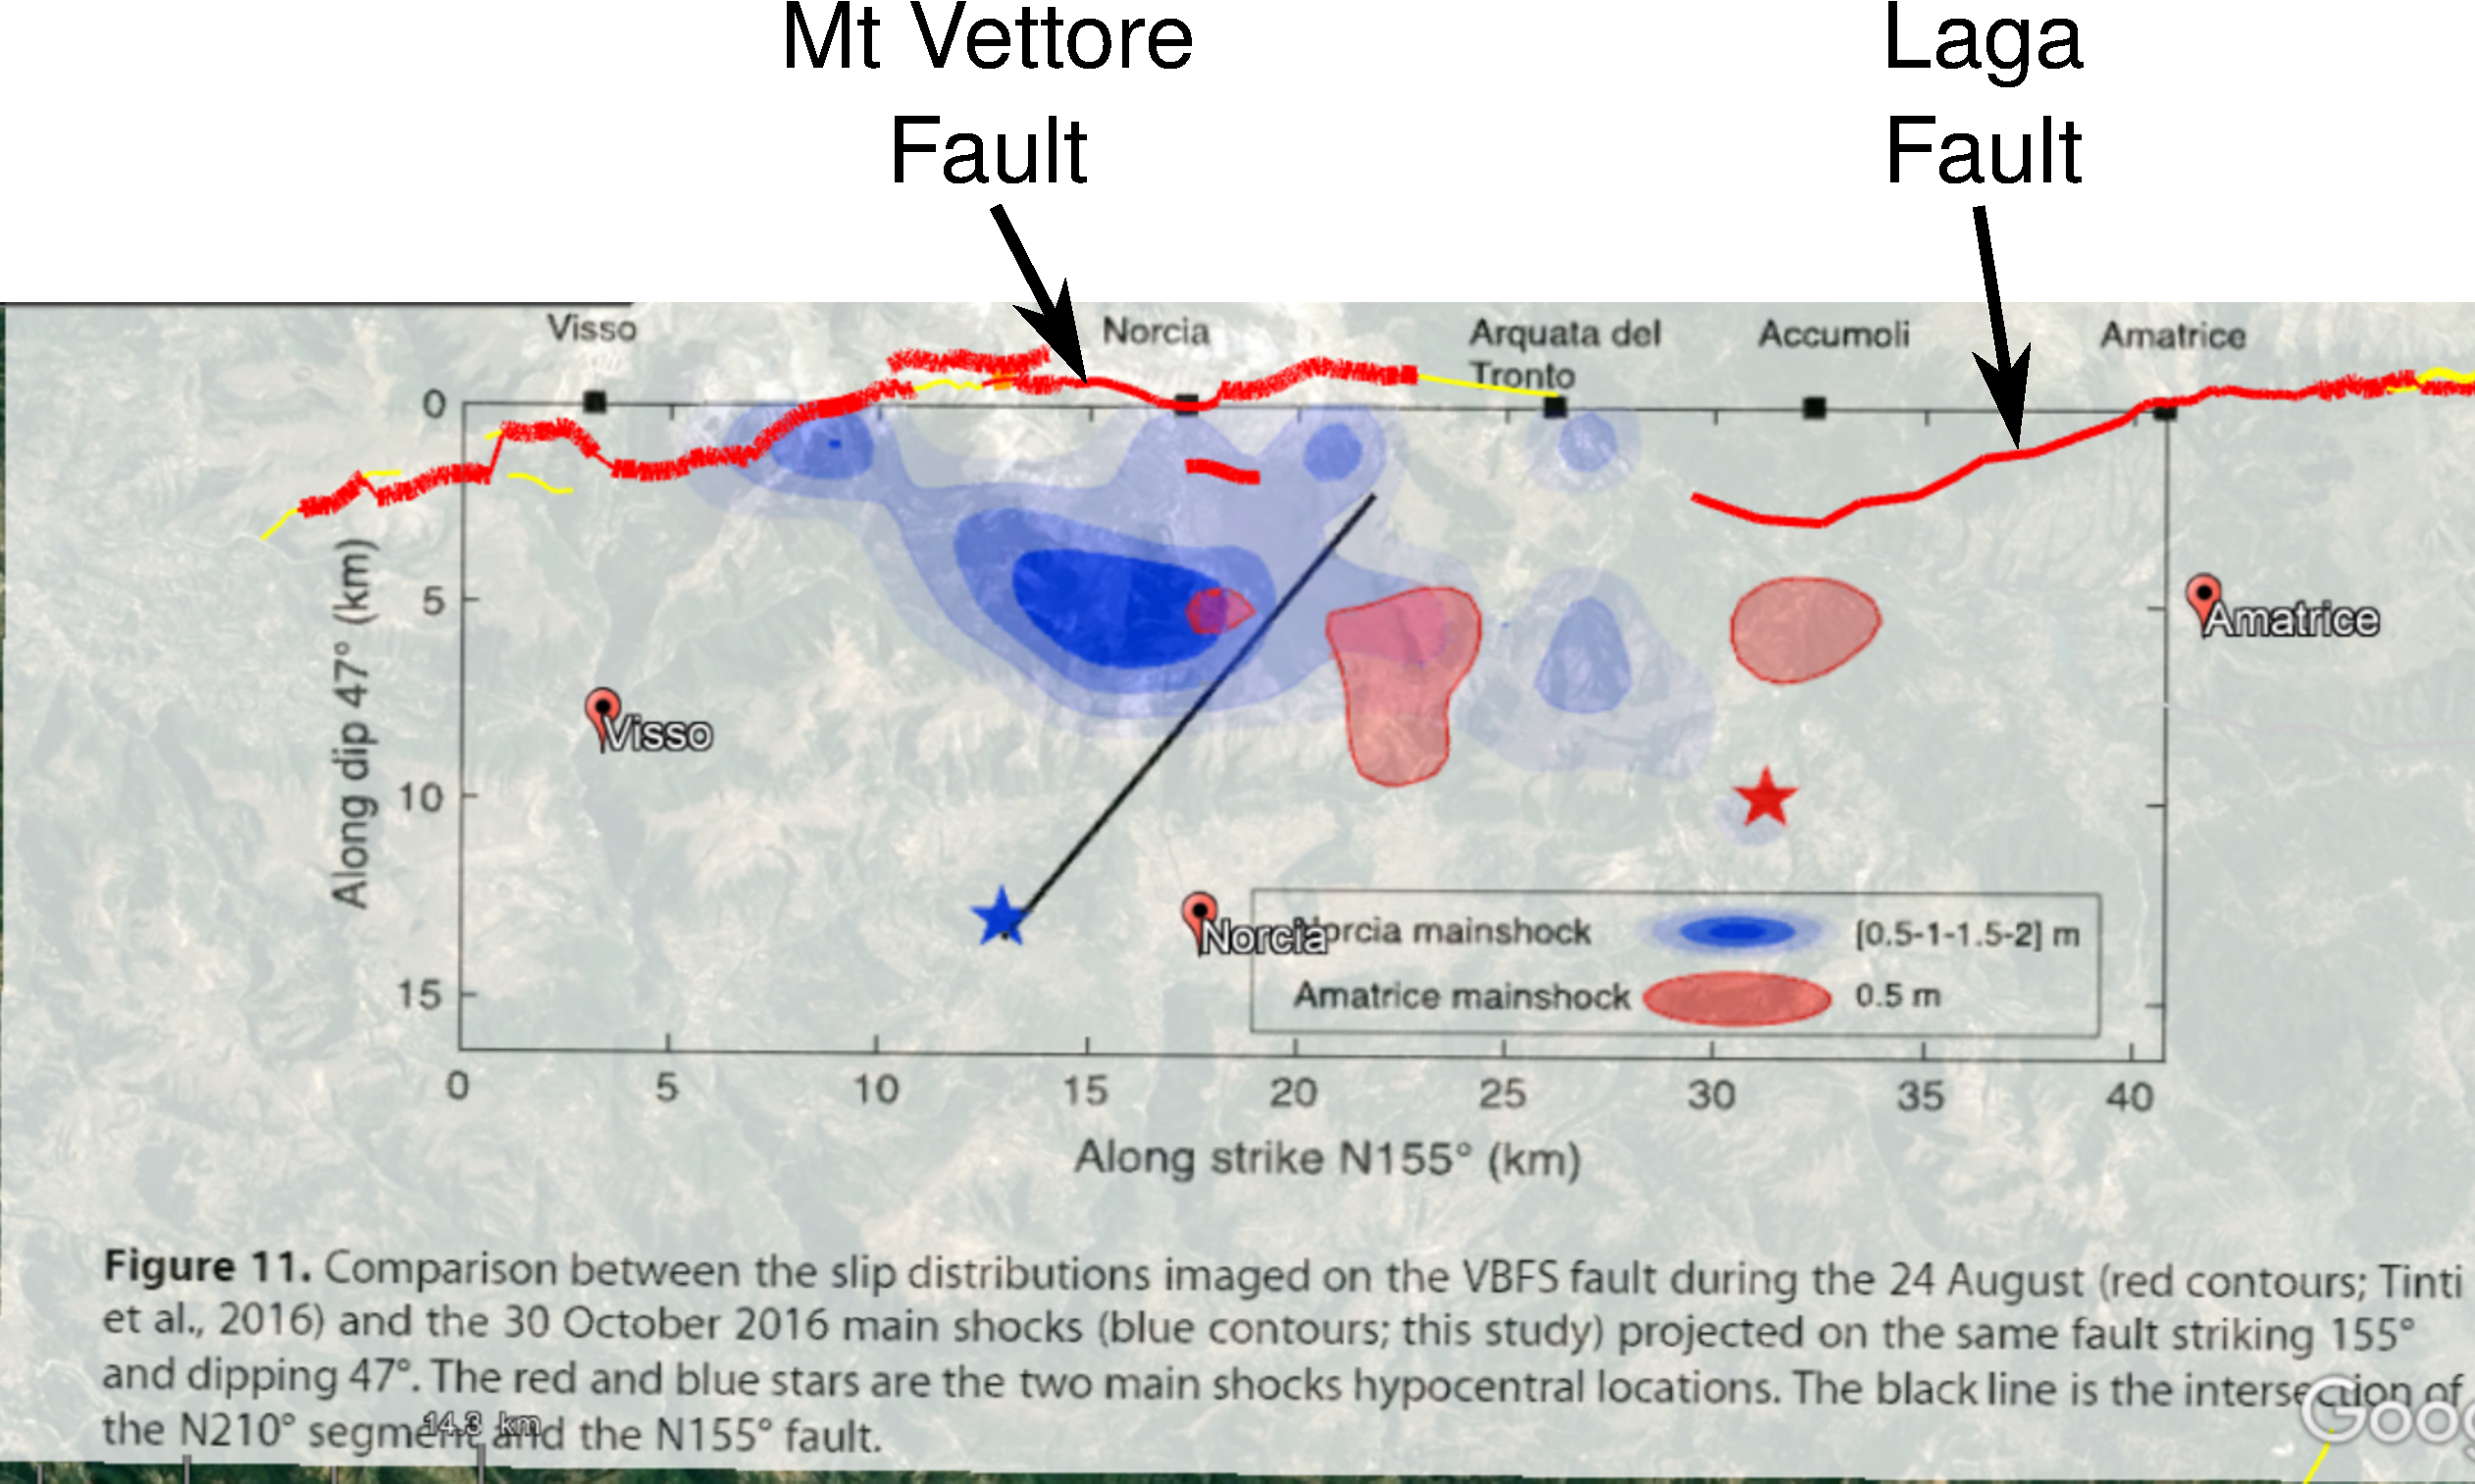
\includegraphics[width=1\linewidth]{images/amatrice_1.pdf} \,
  \vskip 0.2cm
  {\bf \tiny Modified by O. Scotti from \cite{Scognamiglio_2018_CFG}} \end{minipage}
 \begin{minipage}{0.33\linewidth}
  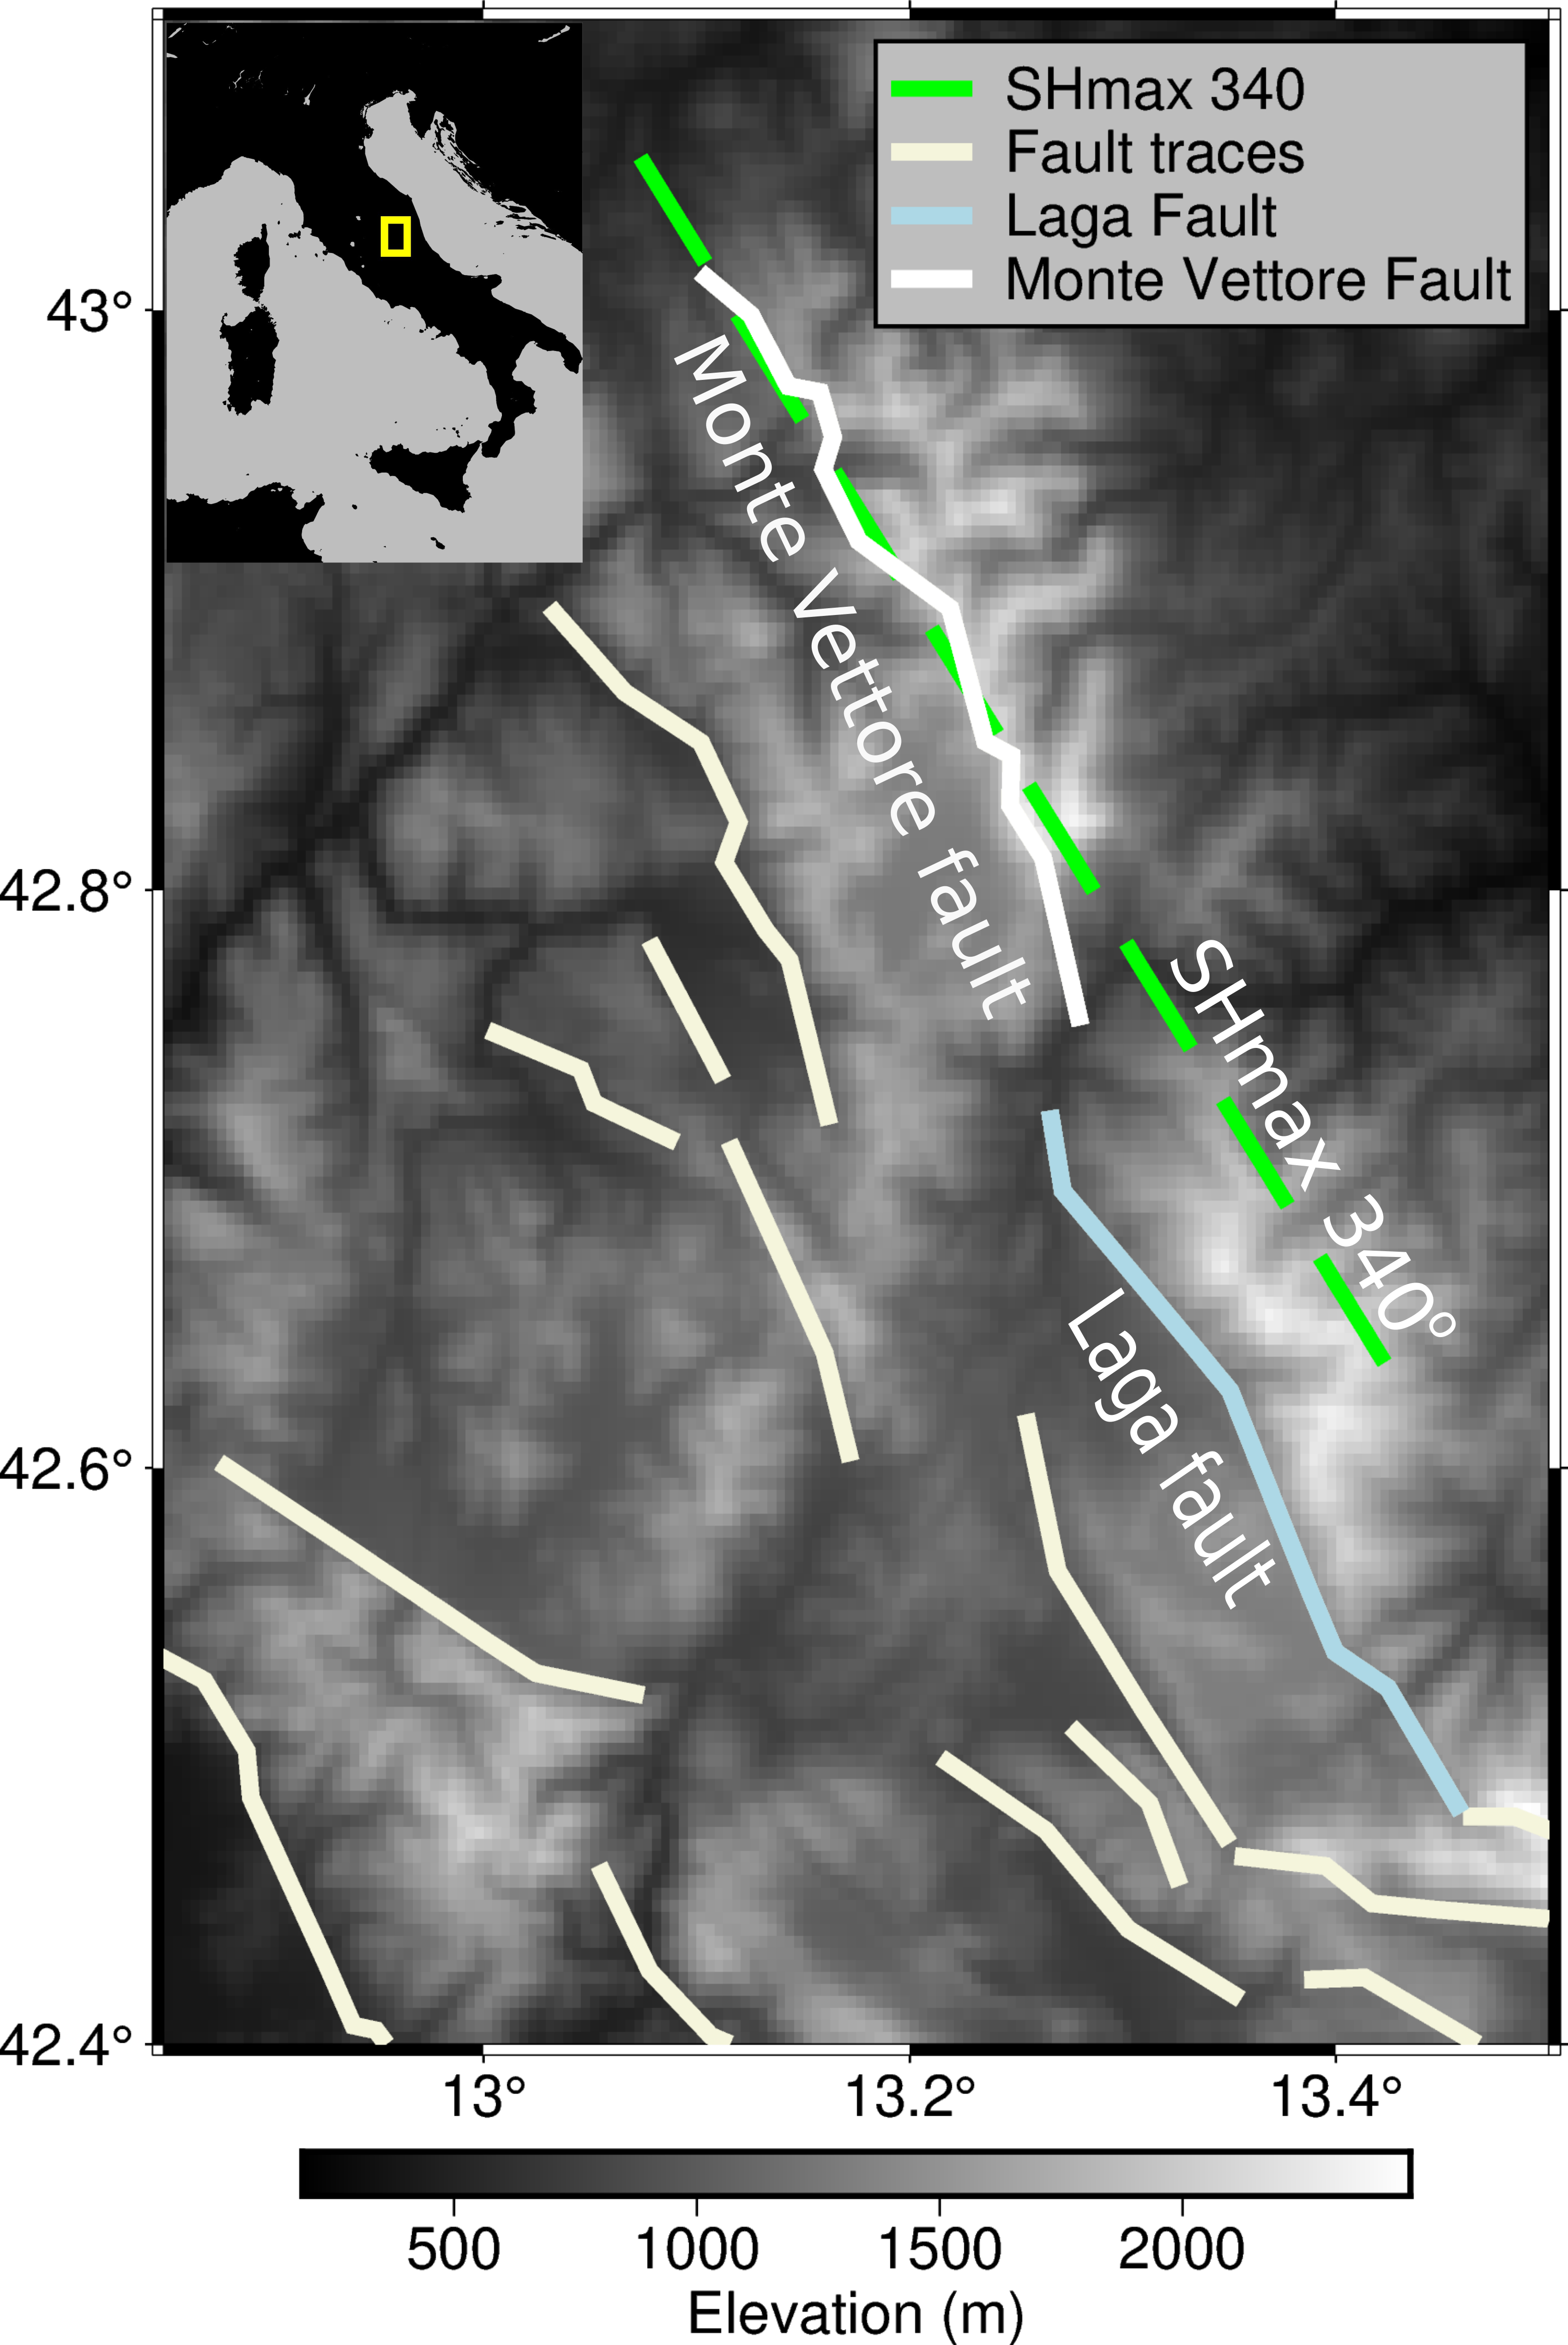
\includegraphics[width=1\linewidth]{images/Map_Italy.png}  
  \vskip 0.2cm
  {\bf \tiny Map based on \cite{Walker_2021_FAULT2SHA}} \end{minipage}
 \end{center}

  
\end{frame}

\begin{frame}
 {Seismic Hazard in Central Italy}
 
 \begin{center}
 \begin{center}
 \begin{minipage}{0.65\linewidth}
  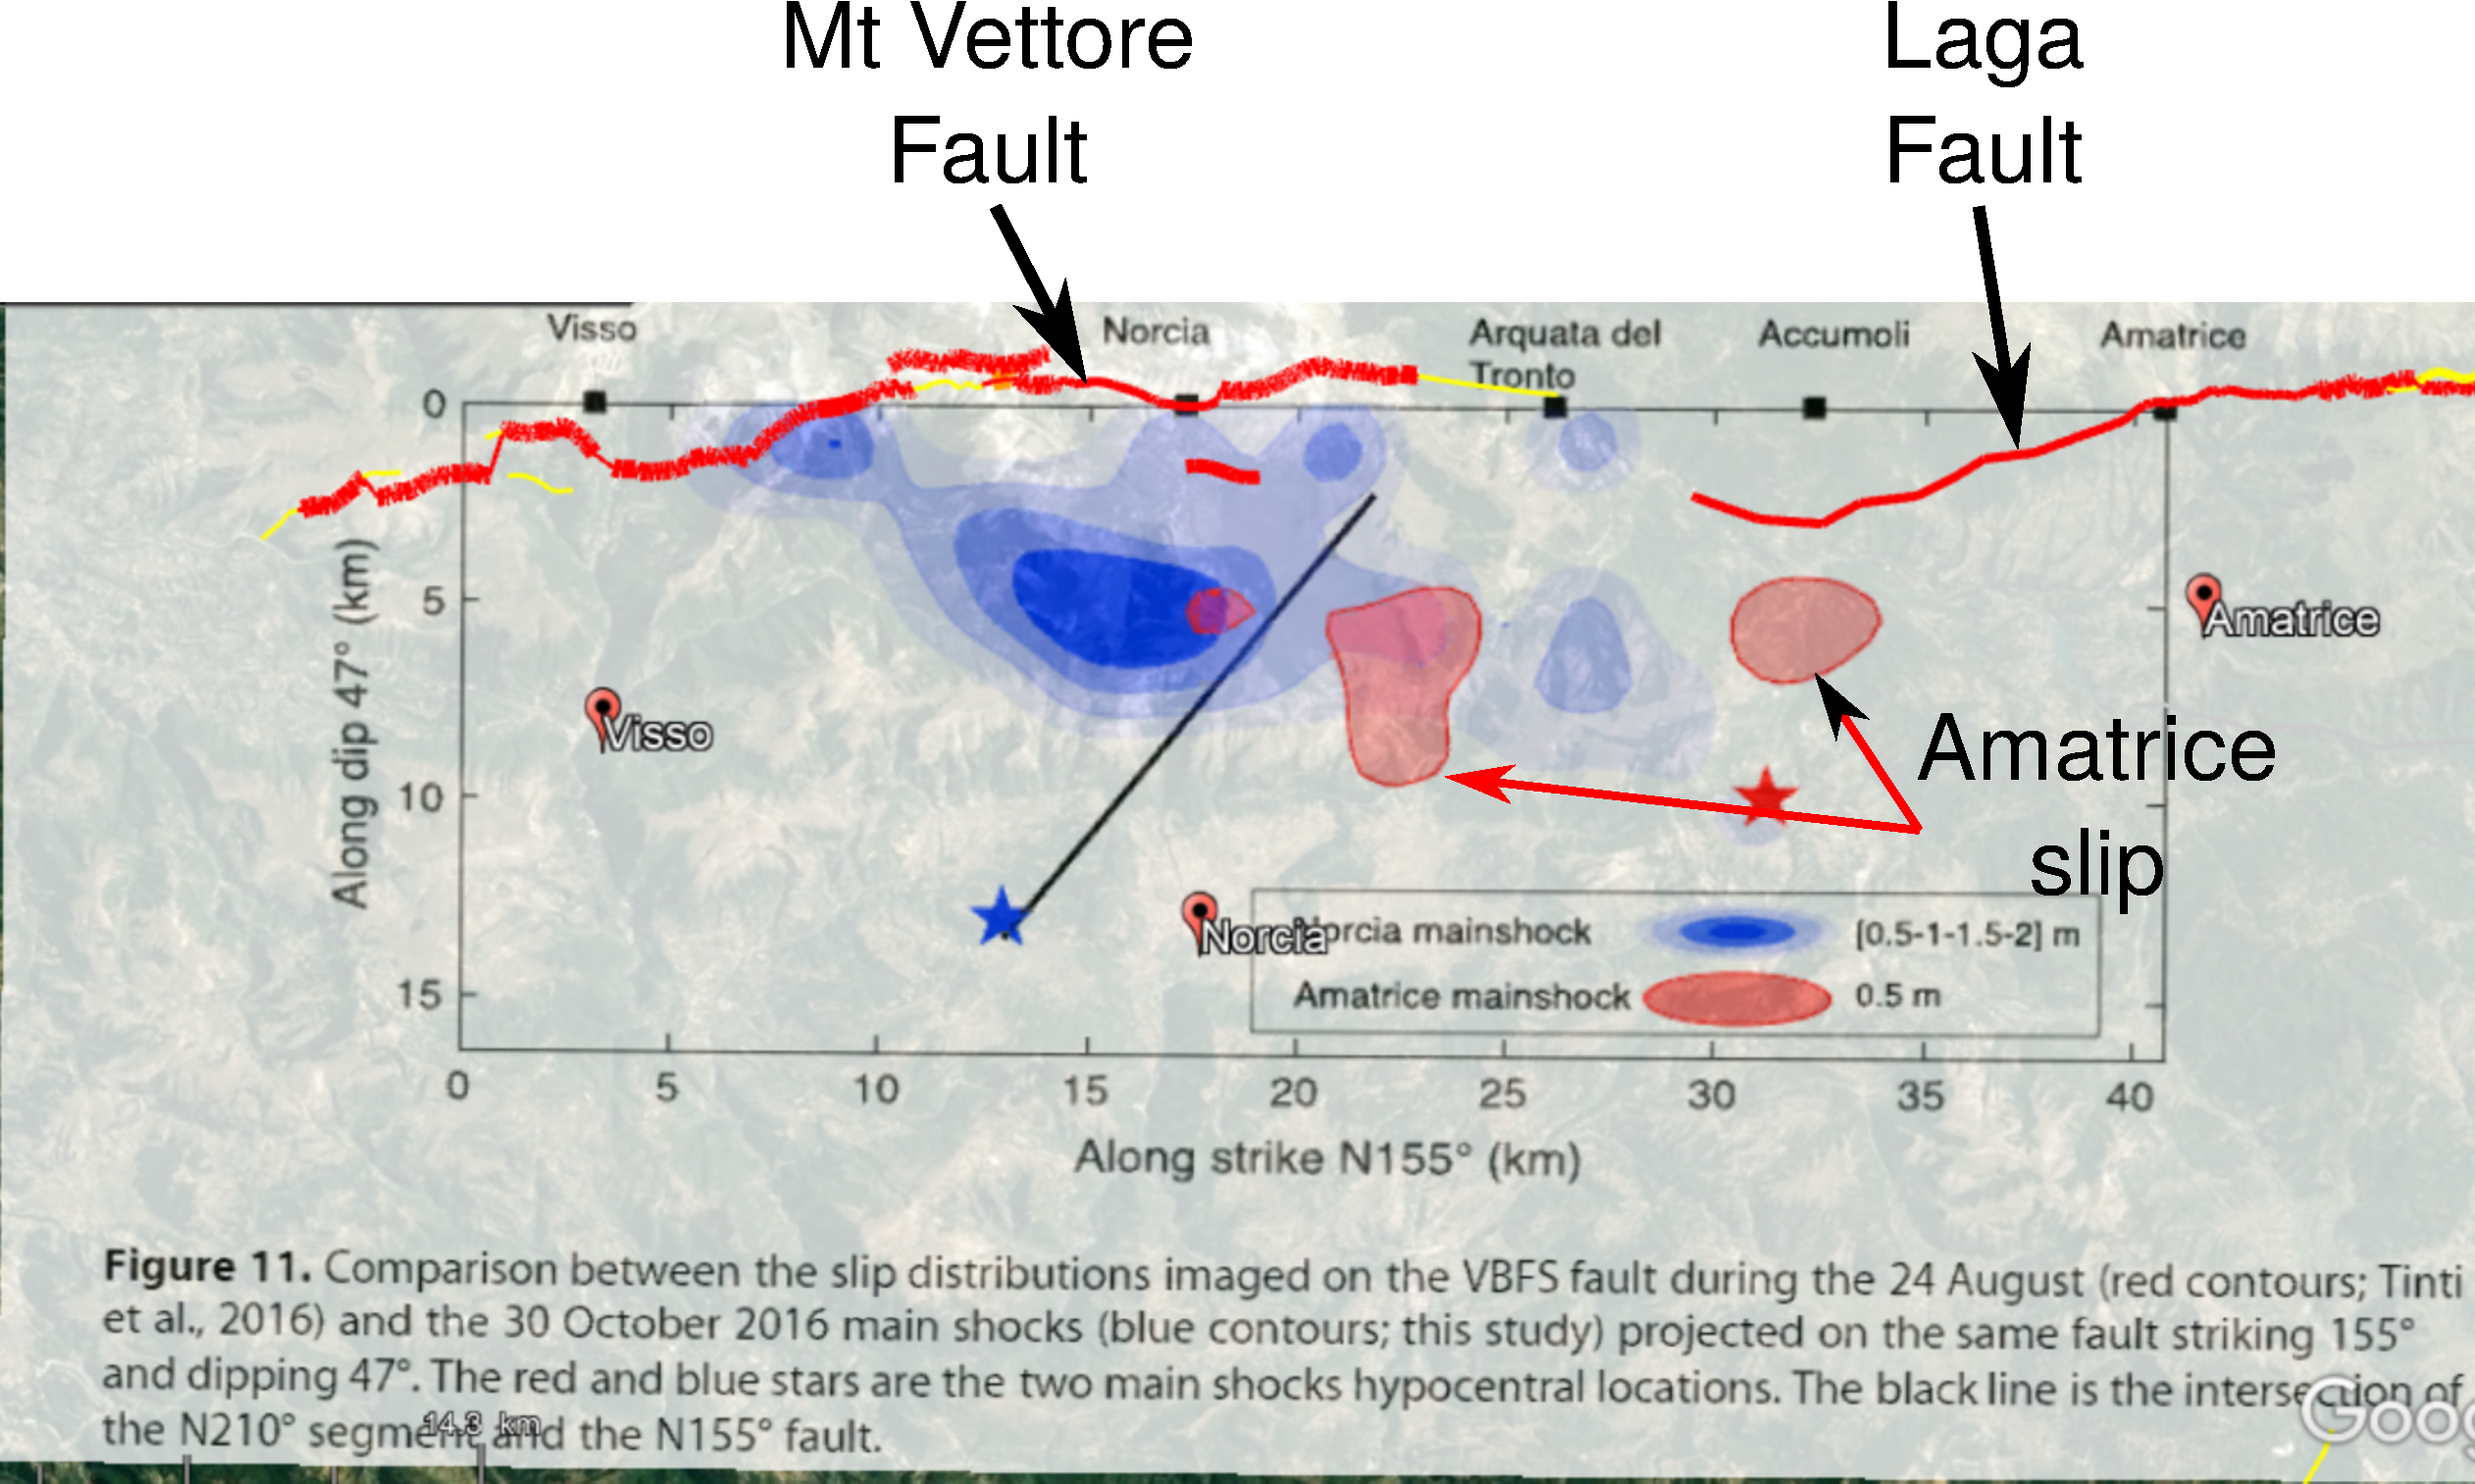
\includegraphics[width=1\linewidth]{images/amatrice_2.pdf} \,
  \vskip 0.2cm
  {\bf \tiny Modified by O. Scotti from \cite{Scognamiglio_2018_CFG}} \end{minipage}
 \begin{minipage}{0.33\linewidth}
  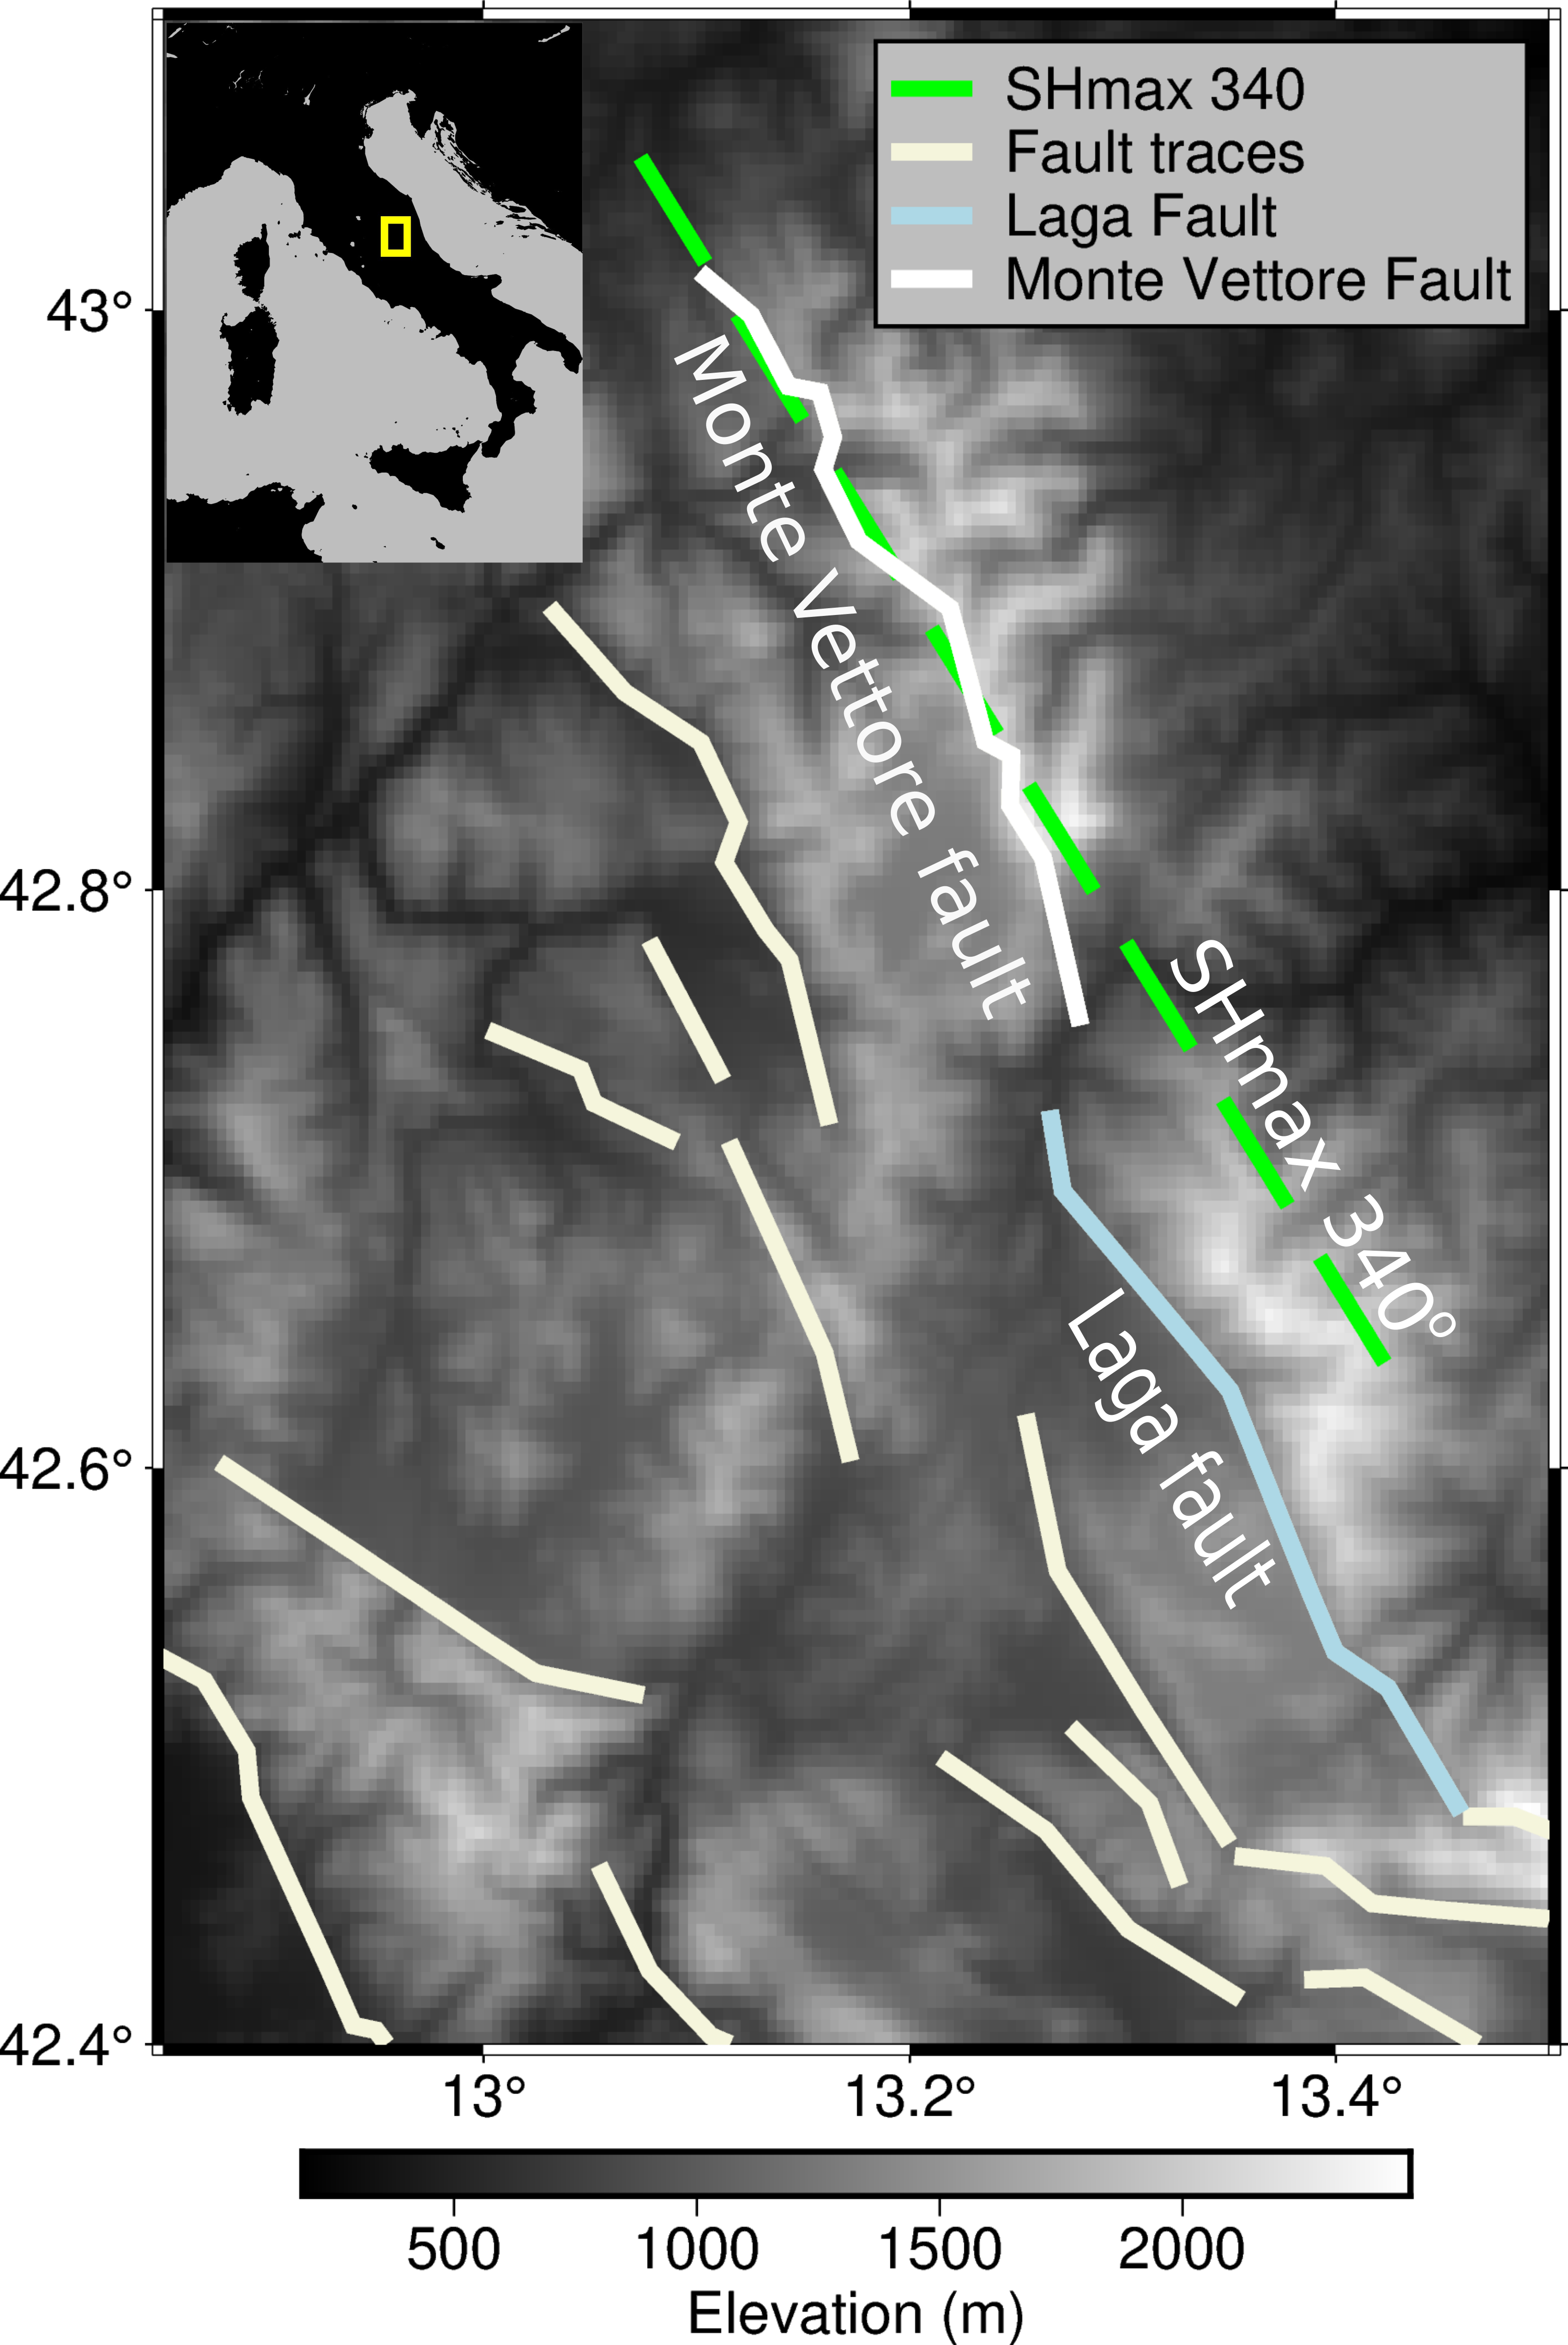
\includegraphics[width=1\linewidth]{images/Map_Italy.png}  
  \vskip 0.2cm
  {\bf \tiny Map based on \cite{Walker_2021_FAULT2SHA}} \end{minipage}
 \end{center}
 \end{center}
  \addtocounter{framenumber}{-1}
  
\end{frame}


\begin{frame}
 {Seismic Hazard in Central Italy}

 \begin{center}
 \begin{center}
 \begin{minipage}{0.65\linewidth}
  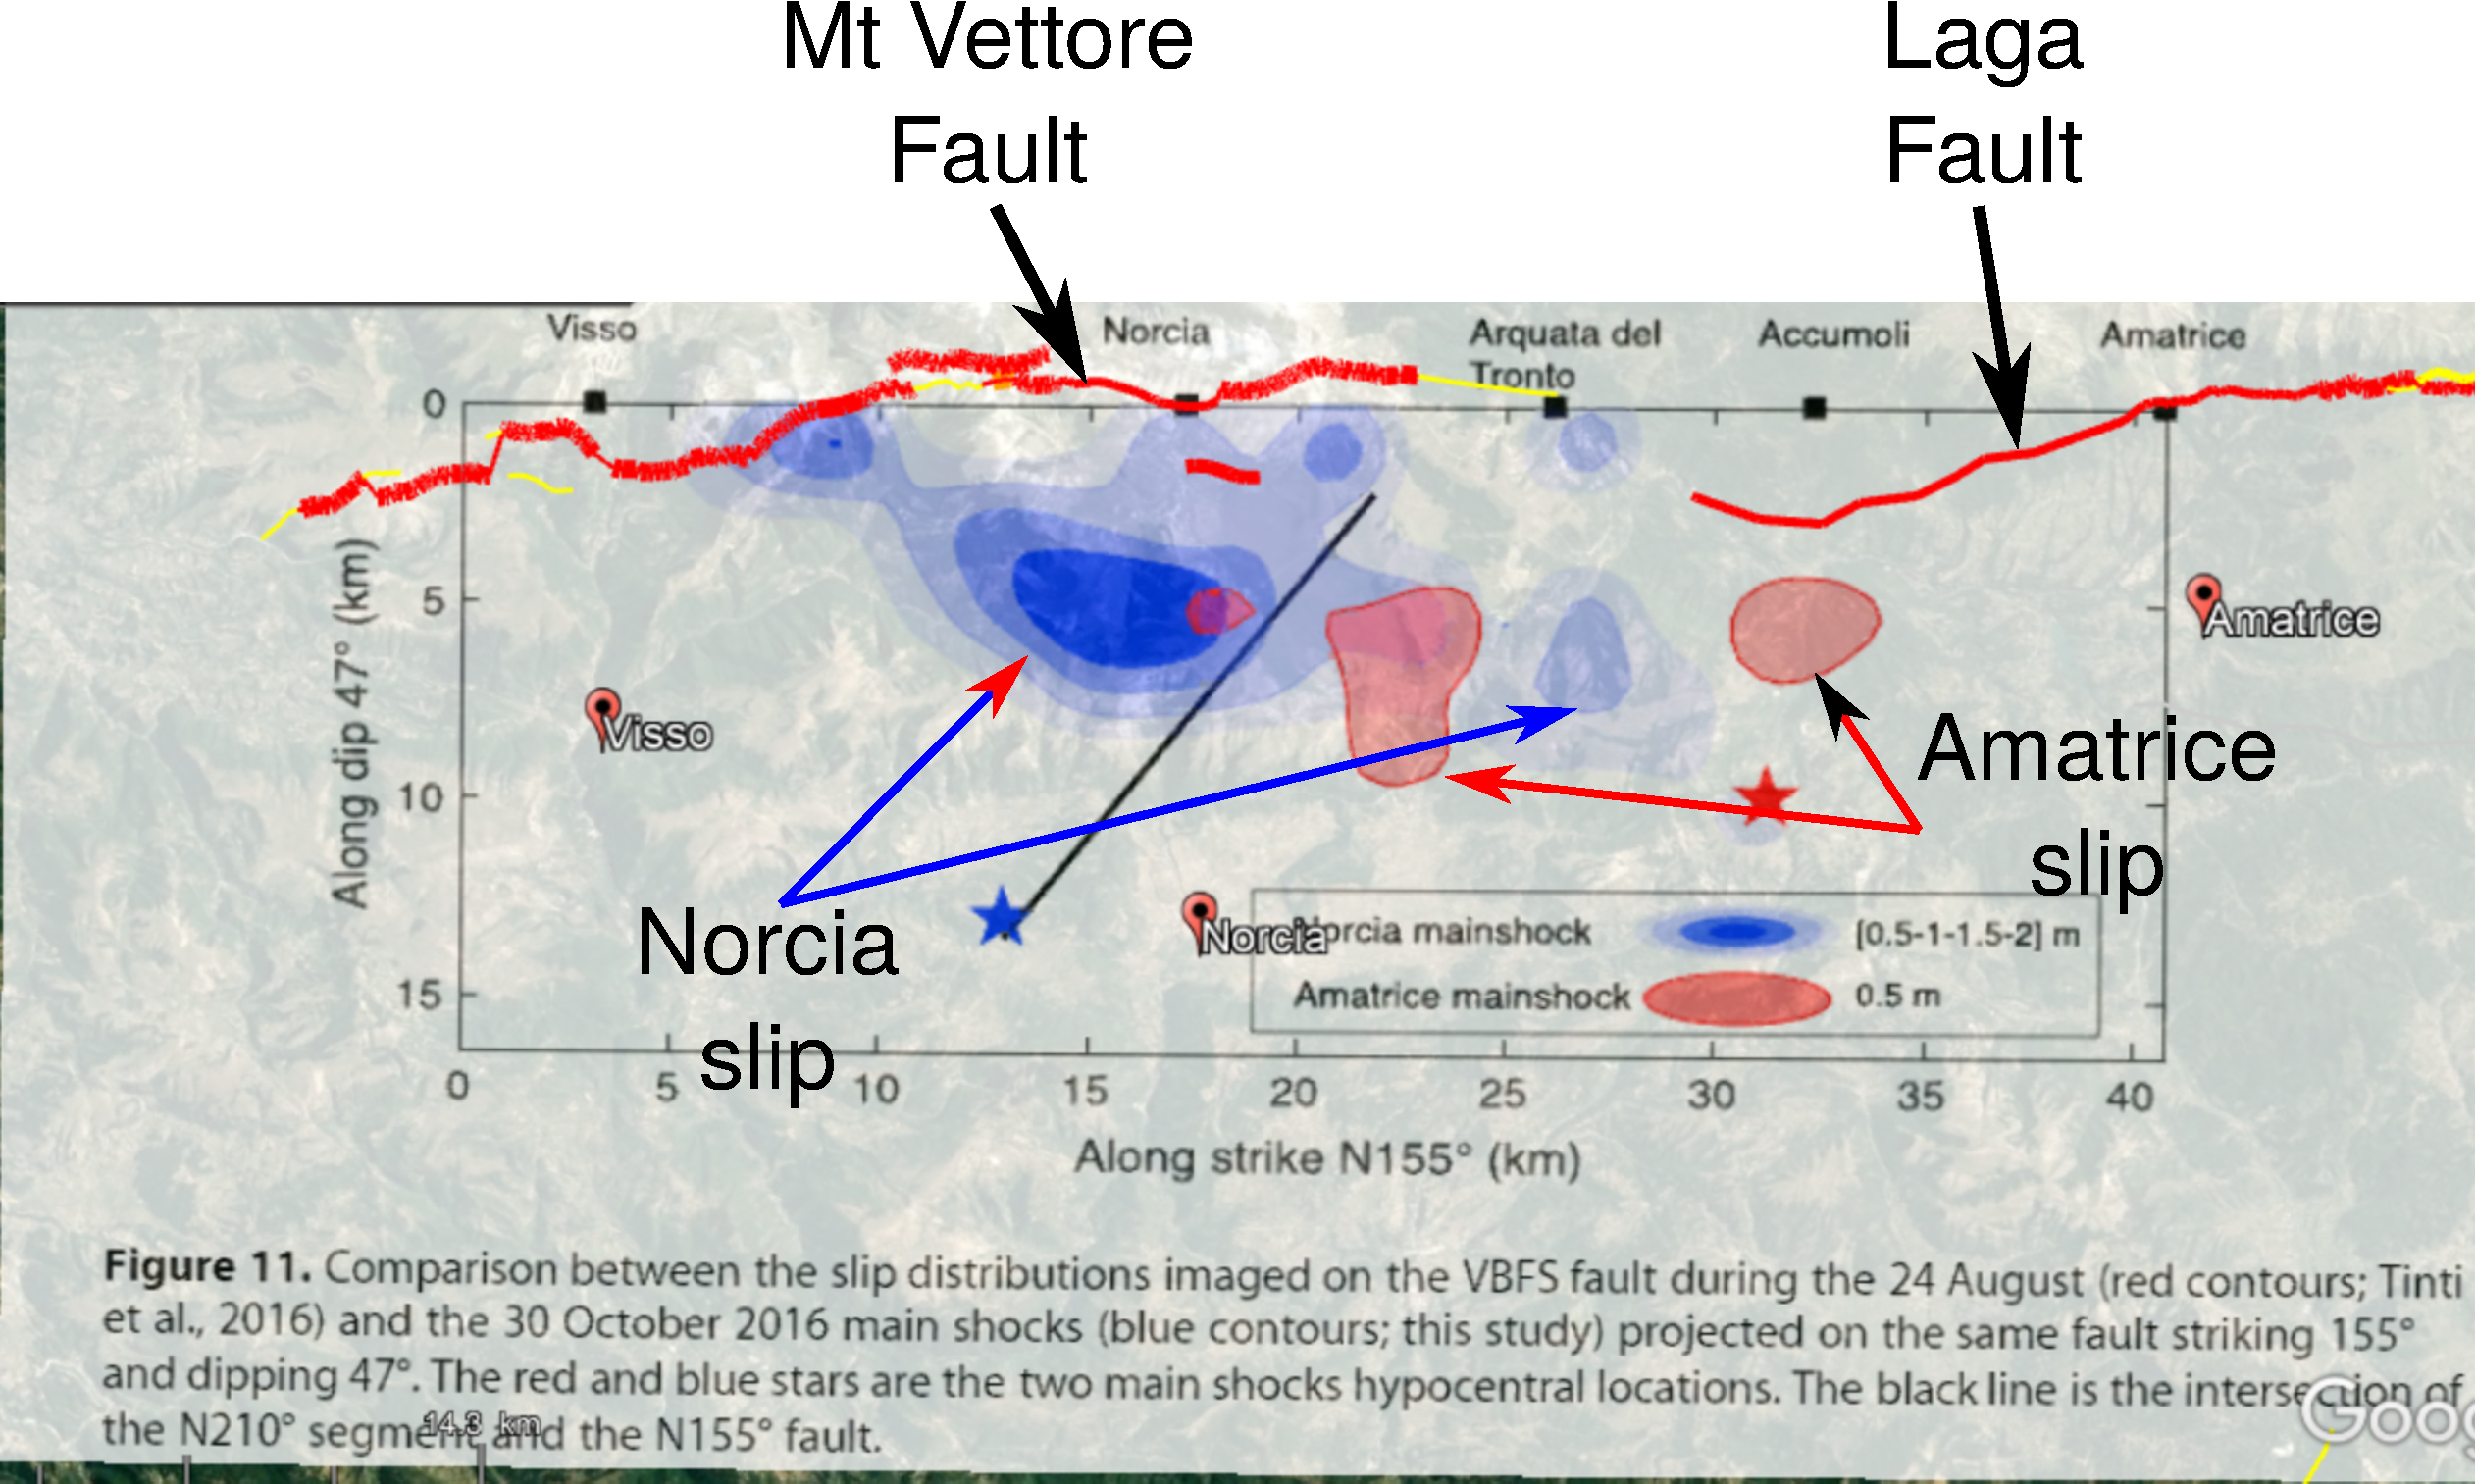
\includegraphics[width=1\linewidth]{images/amatrice_3.pdf} \,
  \vskip 0.2cm
  {\bf \tiny Modified by O. Scotti from \cite{Scognamiglio_2018_CFG}} \end{minipage}
 \begin{minipage}{0.33\linewidth}
  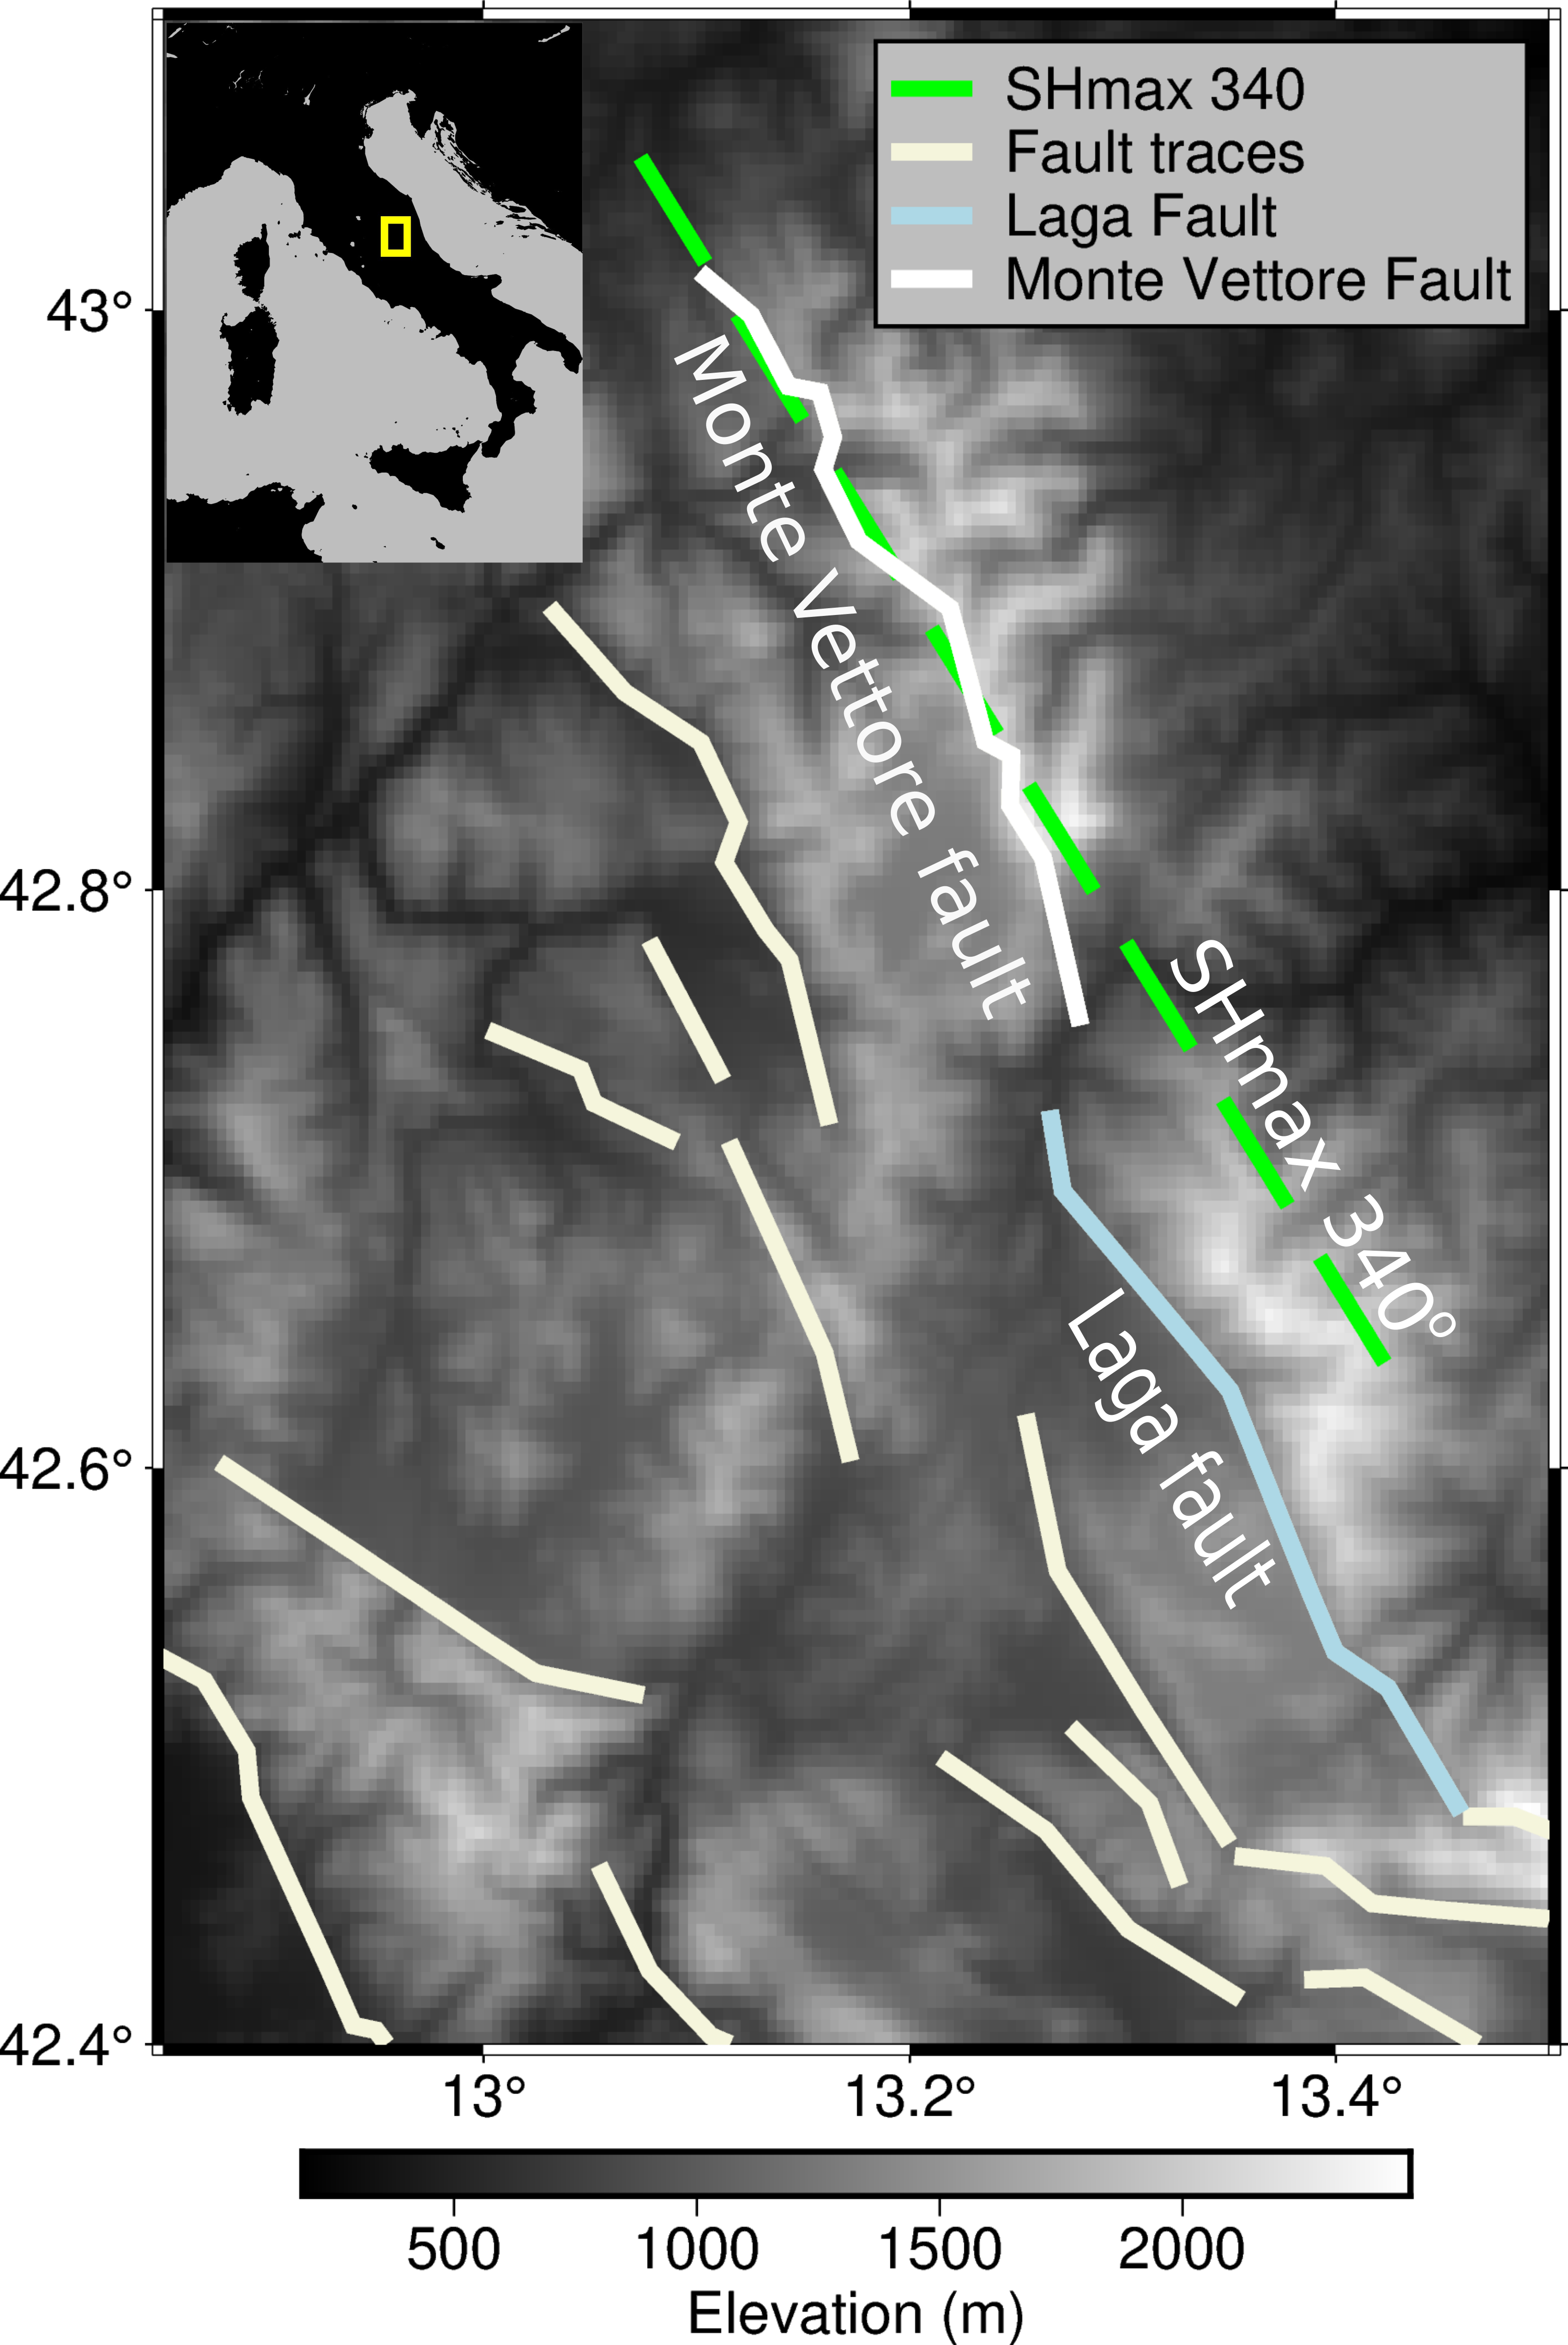
\includegraphics[width=1\linewidth]{images/Map_Italy.png}  
  \vskip 0.2cm
  {\bf \tiny Map based on \cite{Walker_2021_FAULT2SHA}} \end{minipage}
 \end{center}
 \end{center}
  \addtocounter{framenumber}{-1}
  
\end{frame}


\begin{frame}
 {Seismic Hazard in Central Italy}
 
 \begin{center}
  \begin{center}
 \begin{minipage}{0.65\linewidth}
  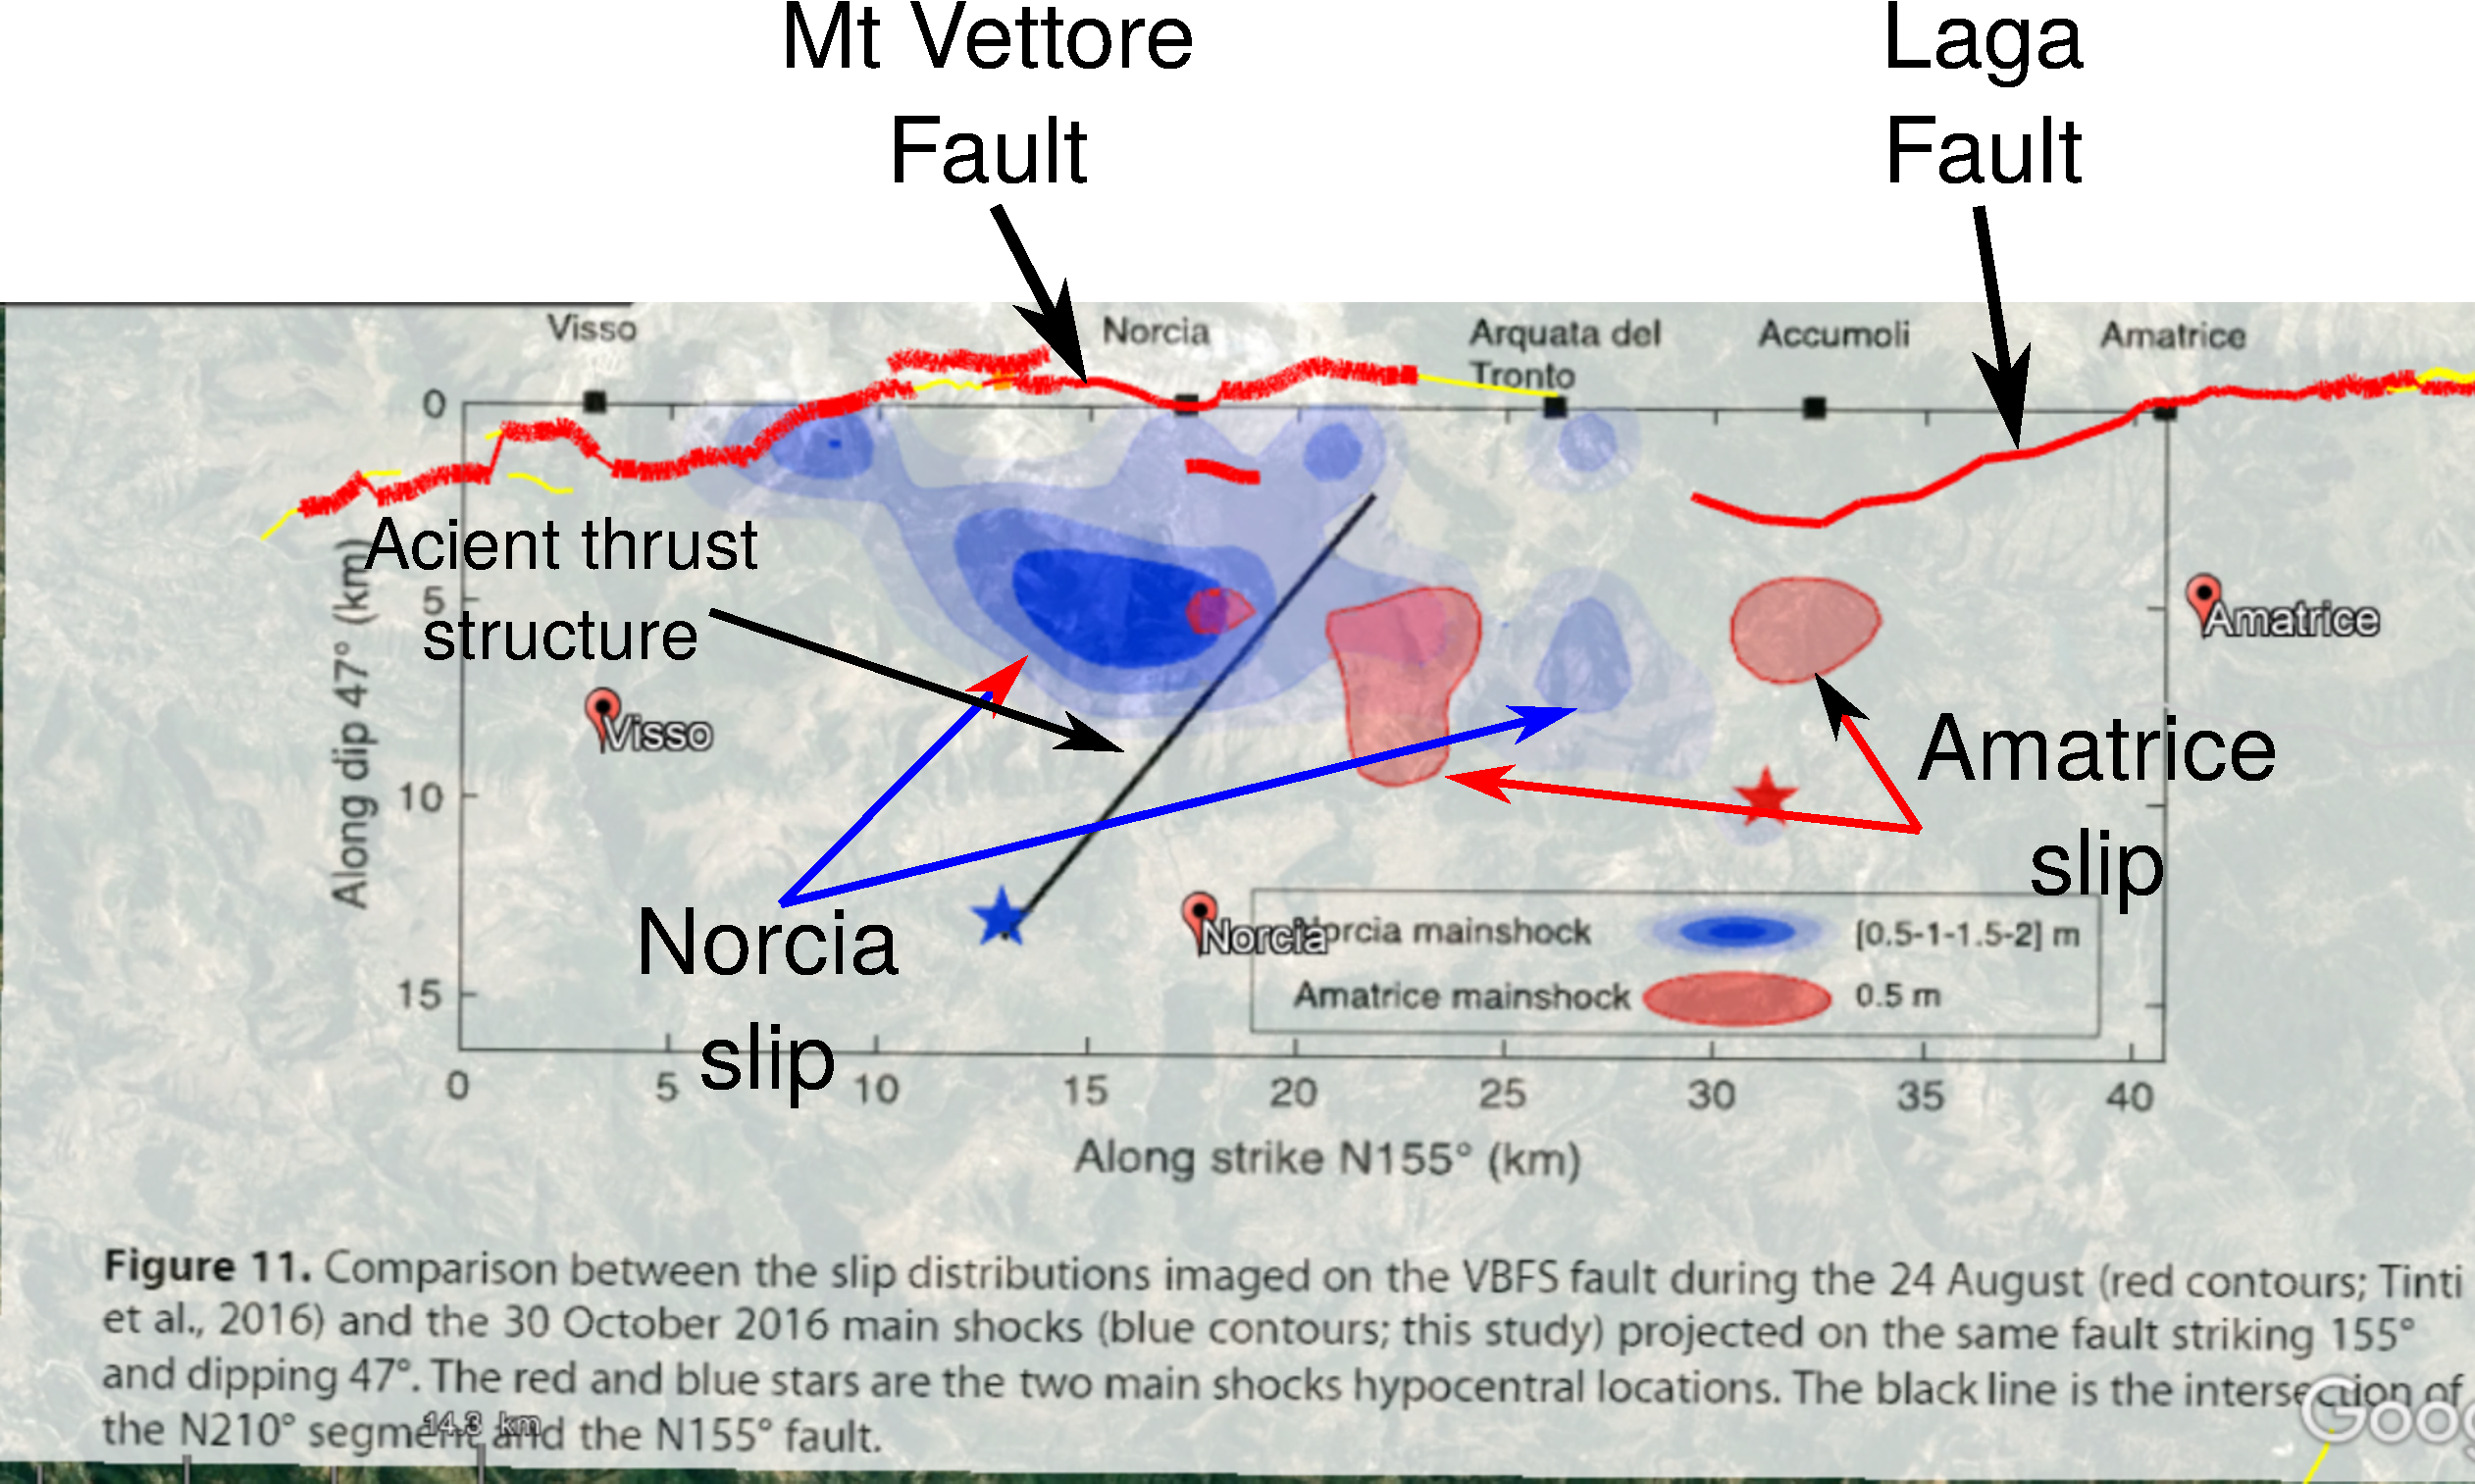
\includegraphics[width=1\linewidth]{images/amatrice_4.pdf} \,
  \vskip 0.2cm
  {\bf \tiny Modified by O. Scotti from \cite{Scognamiglio_2018_CFG}} \end{minipage}
 \begin{minipage}{0.33\linewidth}
  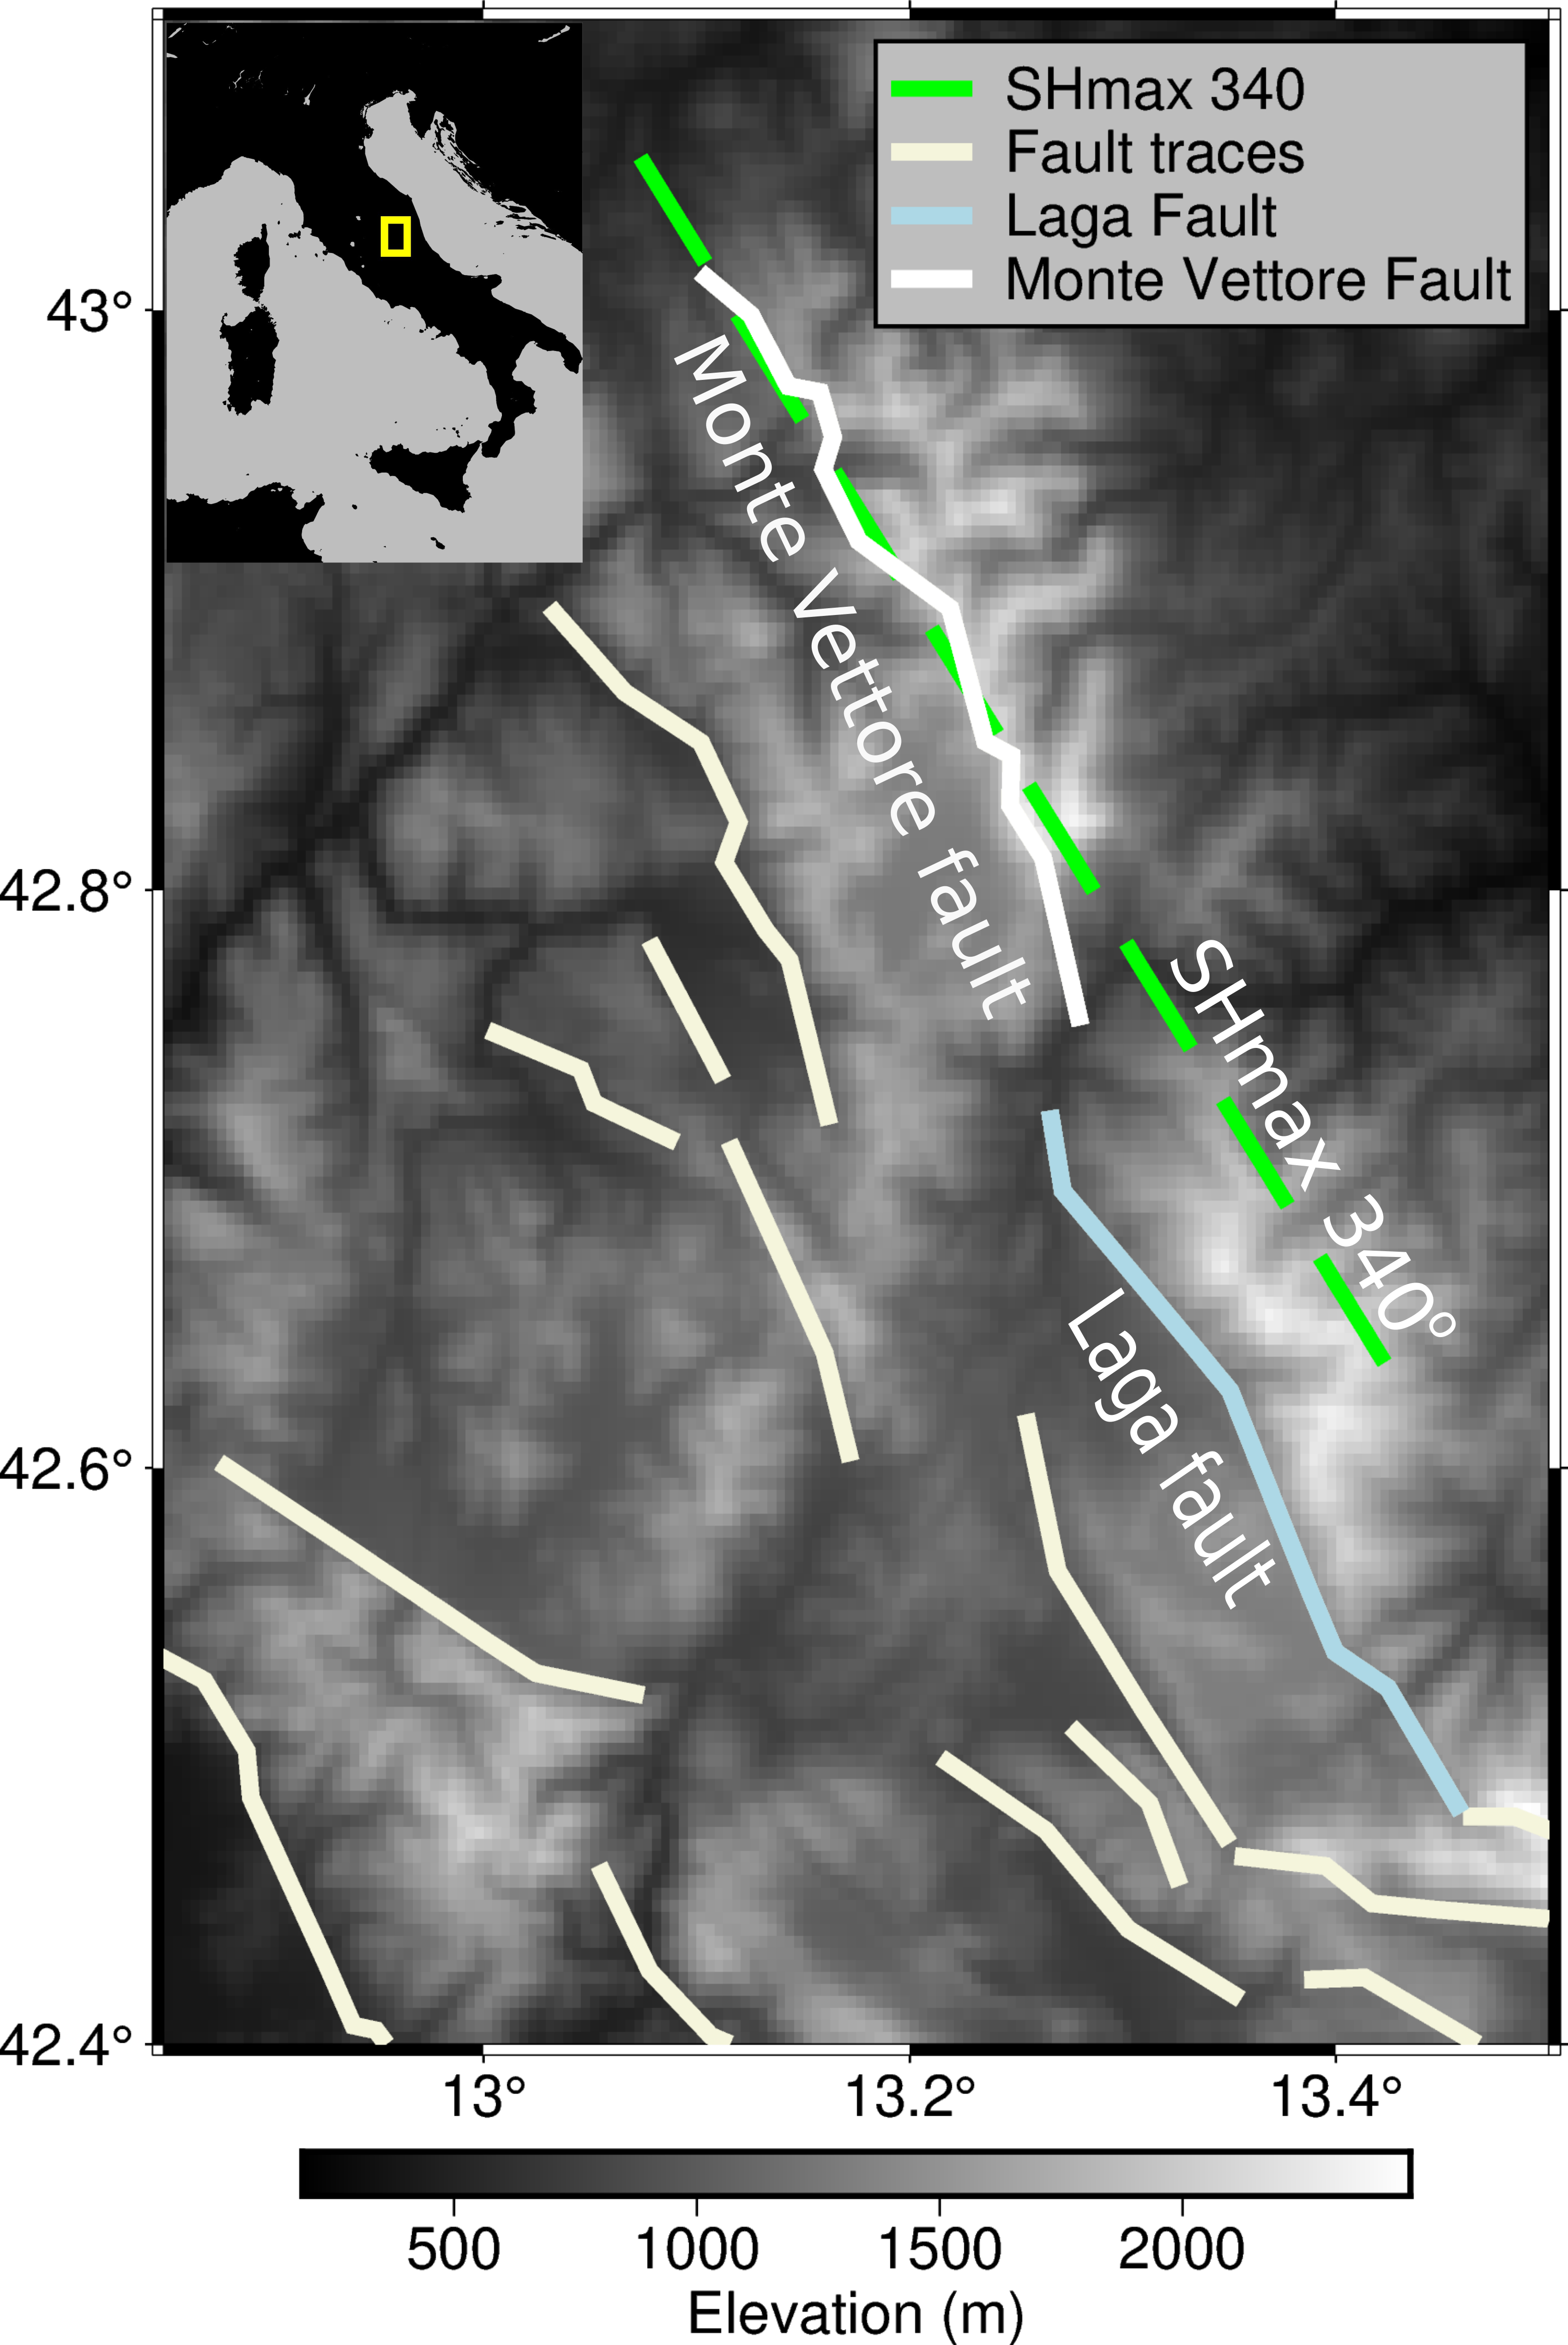
\includegraphics[width=1\linewidth]{images/Map_Italy.png}  
  \vskip 0.2cm
  {\bf \tiny Map based on \cite{Walker_2021_FAULT2SHA}} \end{minipage}
 \end{center}
 \end{center}
  \addtocounter{framenumber}{-1}
  
\end{frame}


\begin{frame}
 {Rupture jumps across step-overs}

  {\scriptsize \textbf{Previous studies focused on strike-slip fault systems:} \cite{Galis_2015_ISS,Hu_2016_IEJ,Bai_2017_ESD,Li_2020_ERT,Oglesby_2008_RTJ}, and more ... } \pause
 \vskip 0.2cm
 \begin{minipage}{0.45\linewidth}
  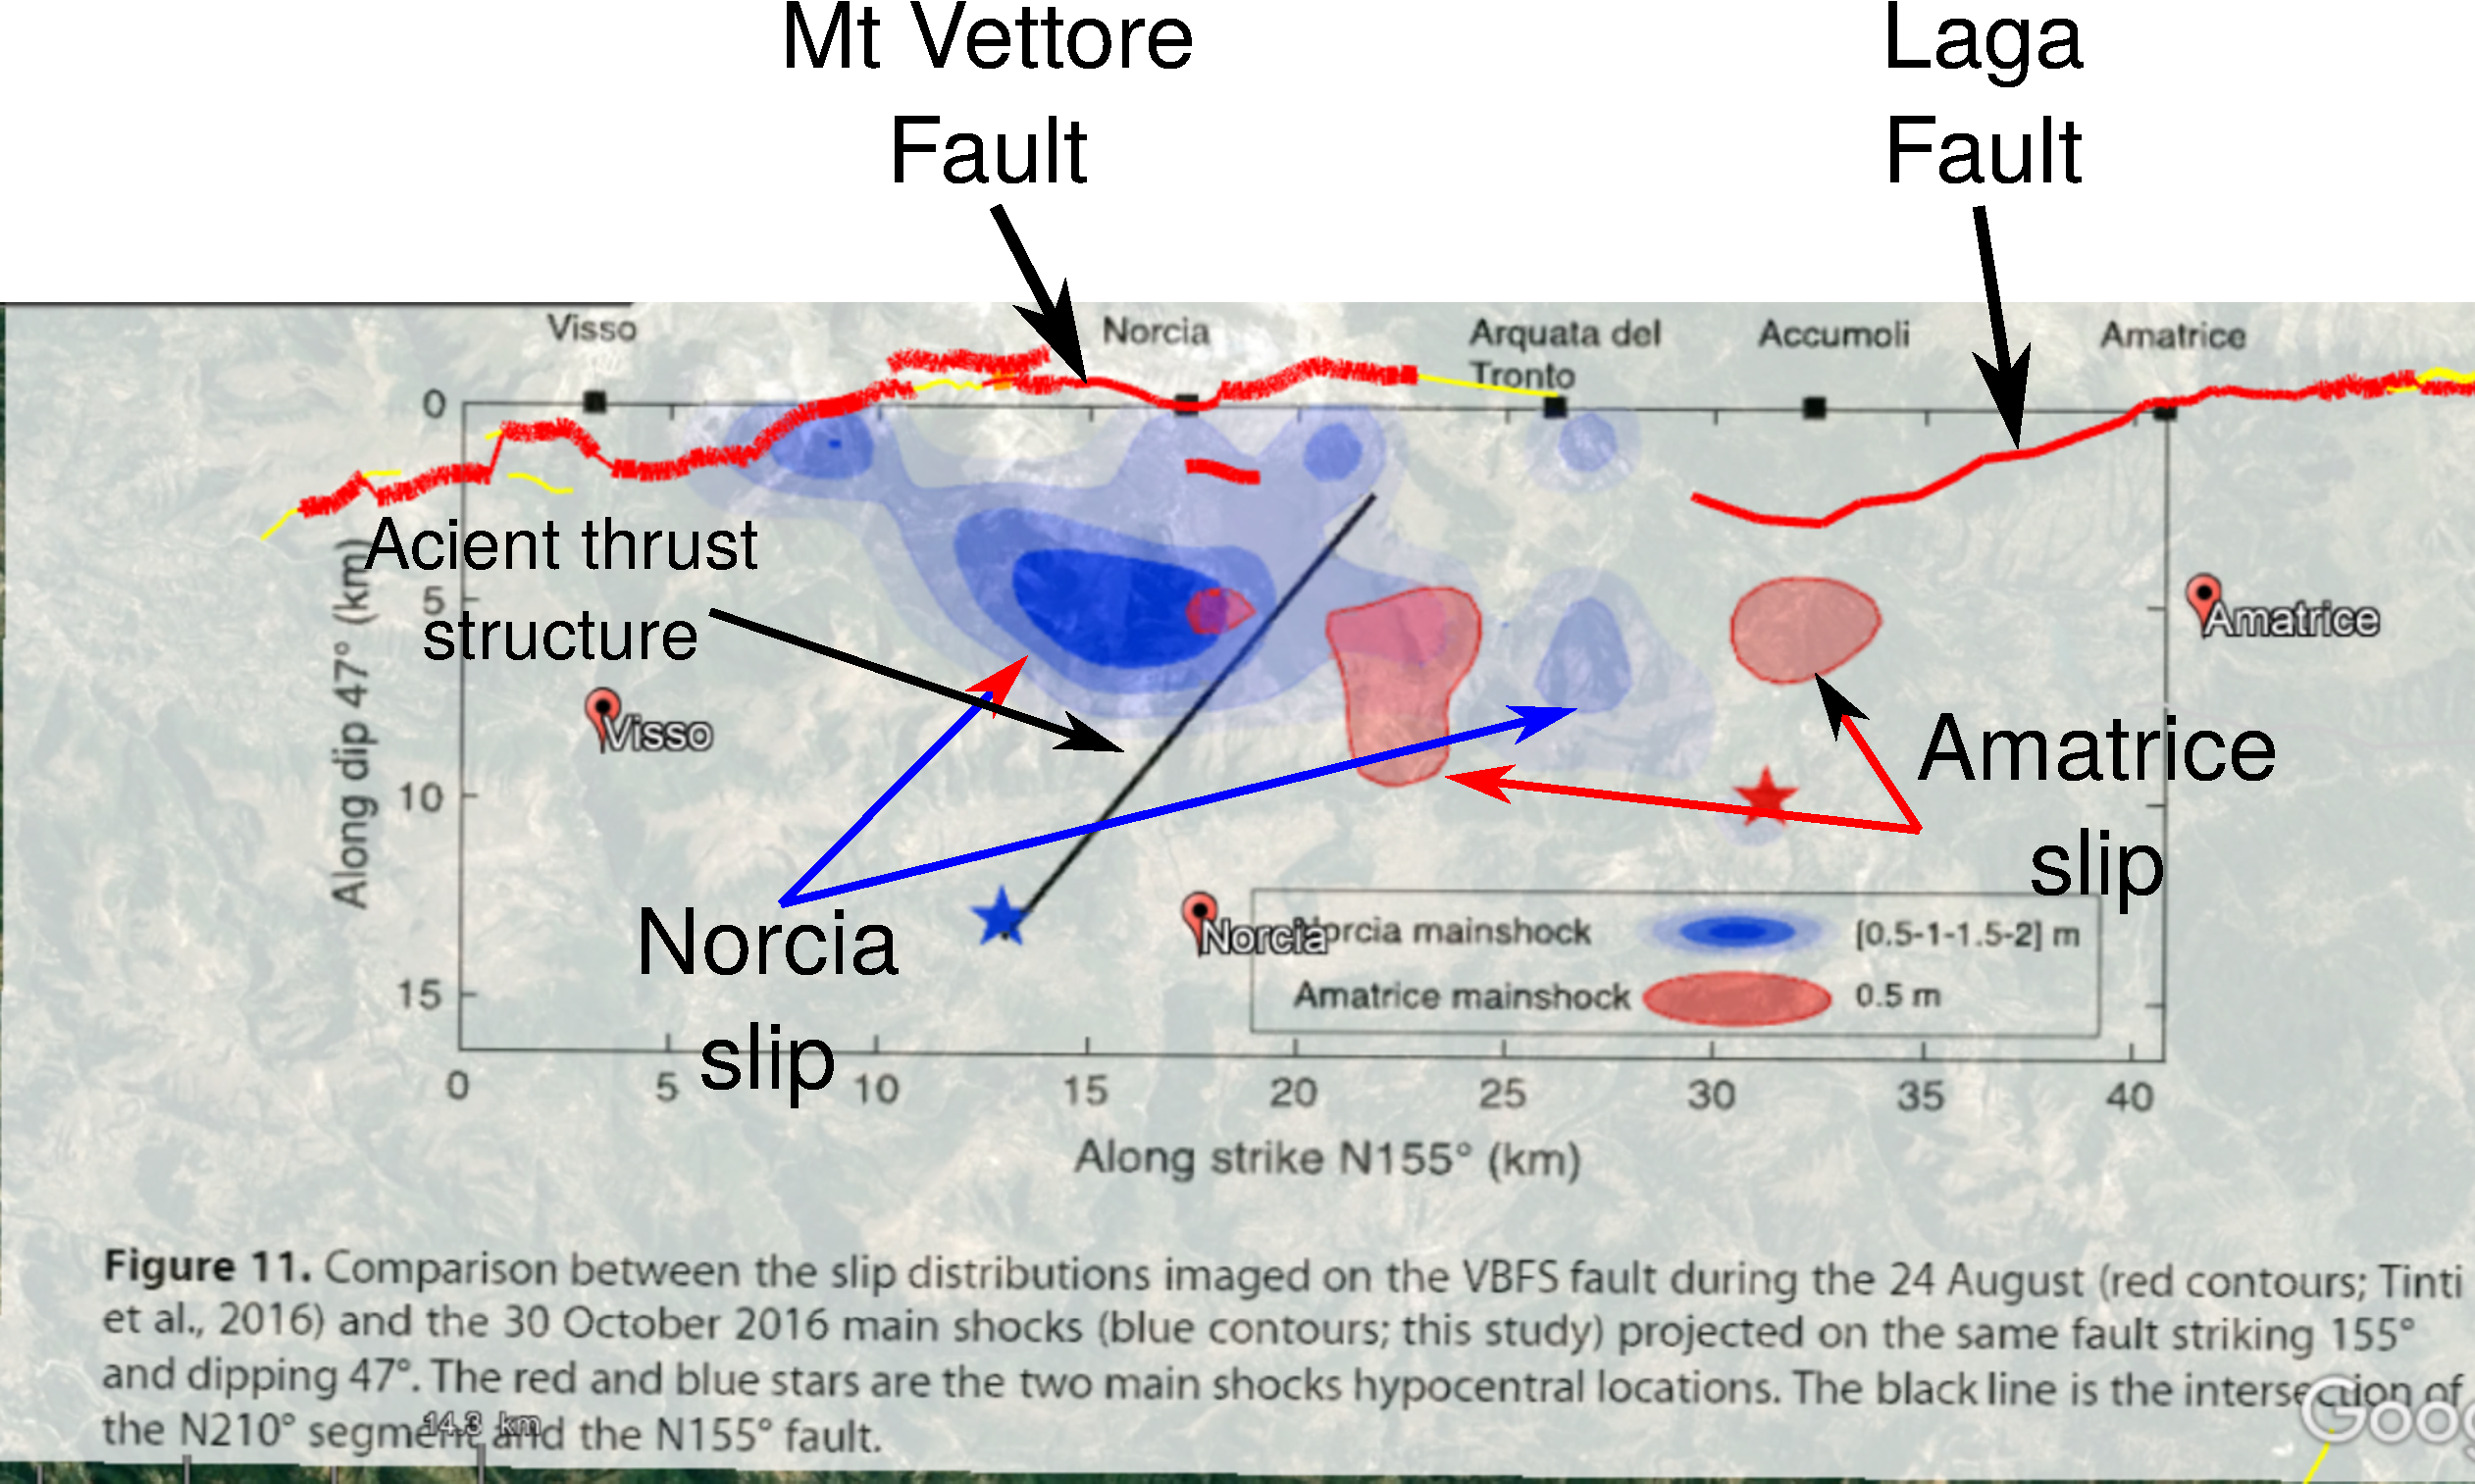
\includegraphics[width=1\linewidth]{images/amatrice_4.pdf}
 \end{minipage}
 \begin{minipage}{0.52\linewidth}
  {\bf \footnotesize In Central Italy:}
  \begin{itemize}
   \footnotesize \item \footnotesize Complex normal faulting systems  \pause
   \footnotesize \item \footnotesize Potential larger magnitudes? \pause
   \item \footnotesize Conditions promoting this? \pause
   \begin{itemize}
   \vskip 0.3cm
    \item \footnotesize Geometry \pause
    \item \footnotesize Stress conditions \pause
   \end{itemize}
   \vskip 0.3cm
   \item \footnotesize To enhance SHA! \pause
  \end{itemize}
 \end{minipage}

 \begin{center}
 \vskip 0.3cm
   \underline{\bf \small Investigate the physical conditons}
   \underline{\bf \small promoting rupture jumps across step overs} 
   \underline{\bf \small regarding normal fault systems} 
  \vskip 0.3cm
  
 \end{center}
 %\addtocounter{framenumber}{-1}
 
\end{frame}




\section{Settings}

\begin{frame}
 {Geometry and parameters explored}

 \vskip -0.2cm
 \centering 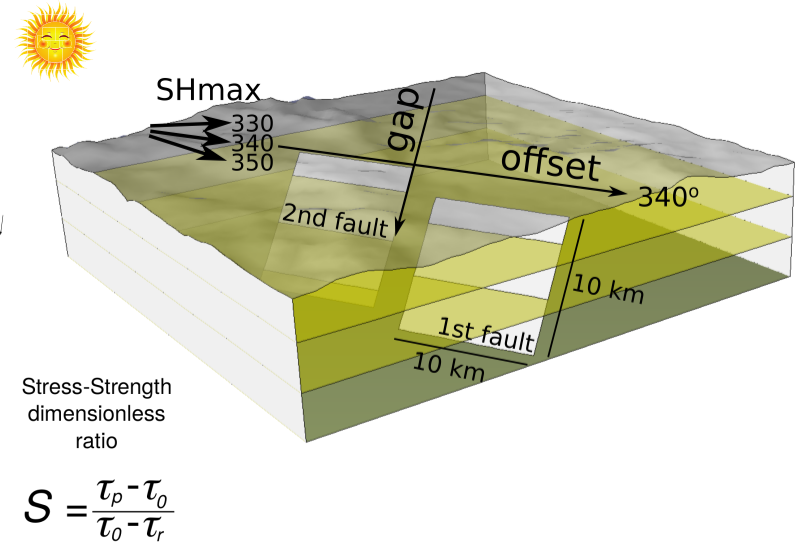
\includegraphics[width=0.9\linewidth]{images/model_no_table_eq}
 \begin{minipage}{0.45\linewidth}
 \vskip -0.3cm
   {\scriptsize Simulations using: www.seissol.org} \\
   \vskip -0.7cm
   {\scriptsize linear slip weakening law} \\   
   \vskip -0.7cm
   {\tiny \citep[e.g.,][]{Wollherr_2018_OFP, Ulrich_2019_CPB}}
 \end{minipage}
 \begin{minipage}{0.45\linewidth}
 \vskip -1.8cm \hskip 2cm \textbf{158 Simulations} \\
 \vskip -1cm
 \hskip 2cm \begin{tabular}{l | r | r | r}
  Parameter           & $\min$ & $\Delta$ & $\max$  \\ \pause
  Offset (km)         & -5     & 2.5      & +5      \\ \pause
  Gap (km)            & -5     & 1        & +5      \\ \pause
  $S$                 & 0.1    & 0.1      & 0.3     \\ \pause
  SH$_{\max}$ ($^o$)  & 330    & 10       & 350     \\ \pause
 \end{tabular}
 \end{minipage}

\end{frame}


\begin{frame}
 {Static analysis ... jump? break-away?}
 
 \begin{center}
 \begin{minipage}{1\linewidth}
  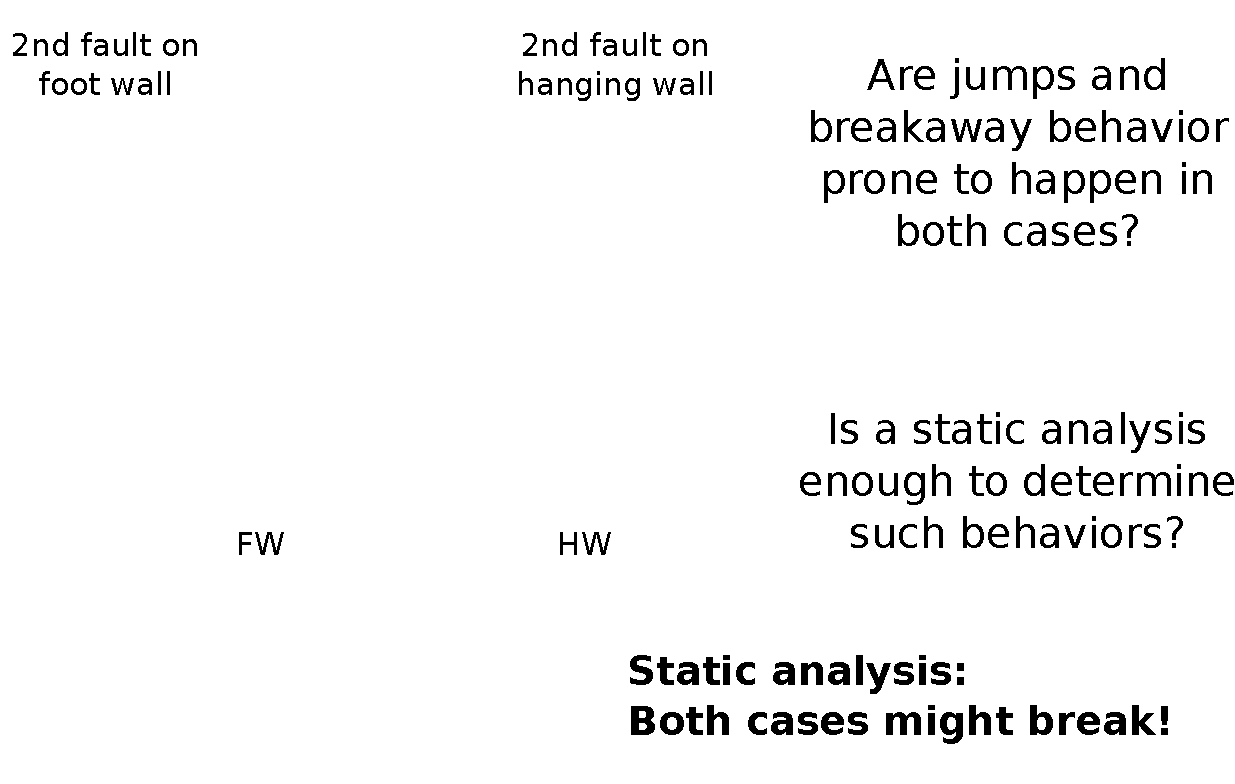
\includegraphics[width=1\linewidth]{images/static_analysis.pdf}
 \end{minipage}
 \end{center}
 
\end{frame}


\section{Results}


\begin{frame}
 {Results ... summary from 158 simulations}
 
 \vskip -0.5cm
  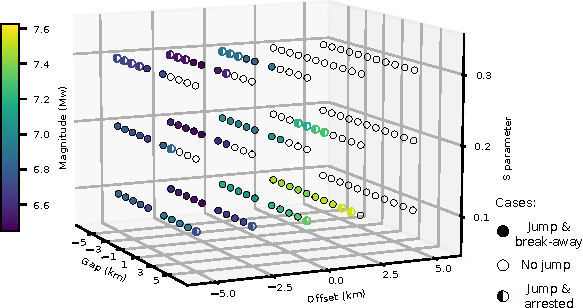
\includegraphics[width=1\linewidth]{images/tests_shmax340}
 
\end{frame}

\begin{frame}
 {Results ... summary from 158 simulations}

  \vskip 0.5cm
  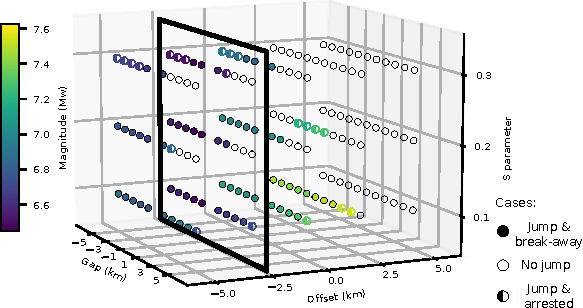
\includegraphics[width=1\linewidth]{images/tests_shmax340_1plane}
  
  \begin{center}
   Let's see in detail some results at \\
   a given offset ... at offset $=-2.5$ km ($\frac{1}{4}$ overlaped) 
  \end{center}

  
   \addtocounter{framenumber}{-1}

\end{frame}


\begin{frame}
 {Results: Hangig/foot wall Asymmetric behavior}
 
 \begin{minipage}{0.45\linewidth}
  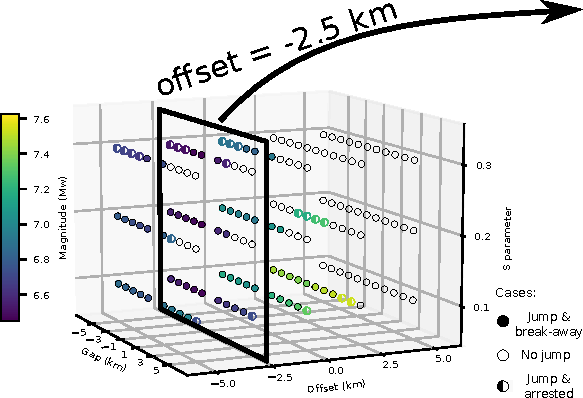
\includegraphics[width=1\linewidth]{images/tests_shmax340_1plane2}
 \end{minipage} \pause
 \begin{minipage}{0.5\linewidth}
  \vskip -0.1cm
  \begin{center}
  \textbf{Compressive/Extensive Asymmetry}
  \vskip 0.2cm
  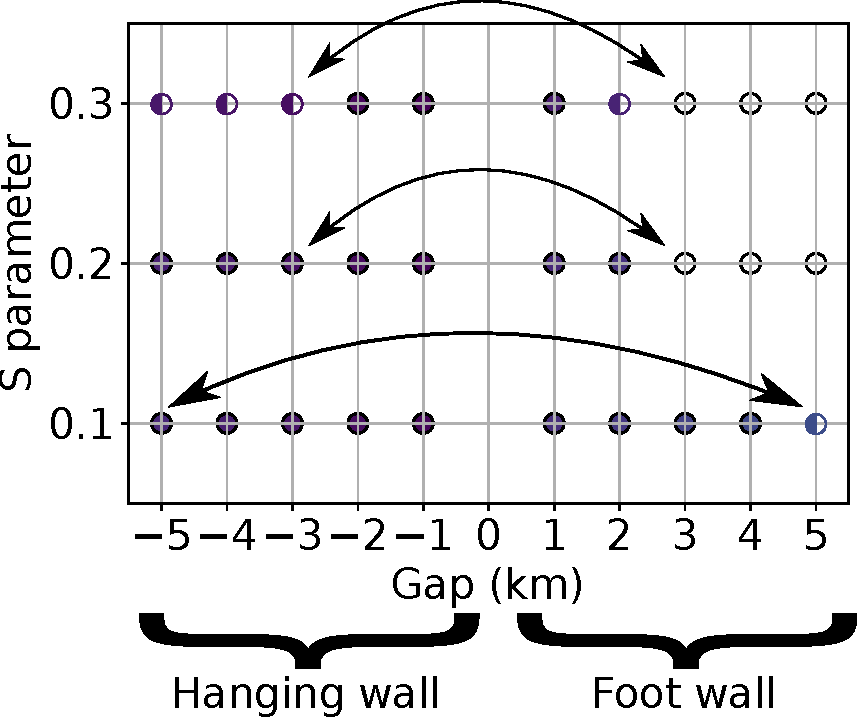
\includegraphics[width=0.9\linewidth]{images/tests_asym} \pause   
  \end{center}
  \vskip -0.3cm
  \begin{itemize}
   \item[\ding{43}] {\scriptsize \textbf{Hanging/foot wall asymmetry:} \\
                    When the 2nd fault is on the hanging wall 
                    (Gap $<$ 0), the rupture is more likely to }
                    \begin{itemize}
                     \item \scriptsize be triggered
                     \item \scriptsize be sustained
                    \end{itemize}
  \end{itemize}
 \end{minipage}
  
\end{frame}


\begin{frame}
 {Results: Stress shadow \ding{43} expected magnitudes}
 
 \begin{minipage}{0.45\linewidth}
  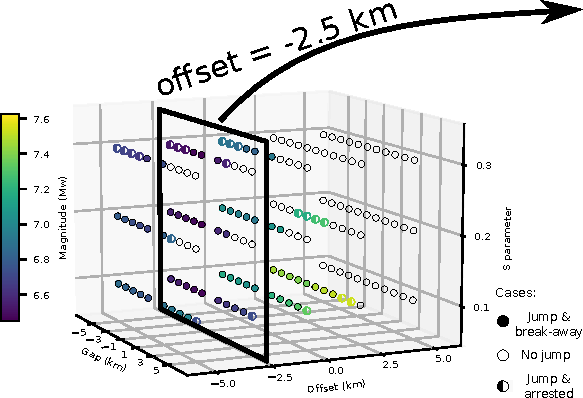
\includegraphics[width=1\linewidth]{images/tests_shmax340_1plane2}
 \end{minipage} \pause
 \begin{minipage}{0.53\linewidth}
  \vskip -0.1cm
  \begin{center}
  \textbf{Proximity VS magnitude}
  \vskip 0.4cm
  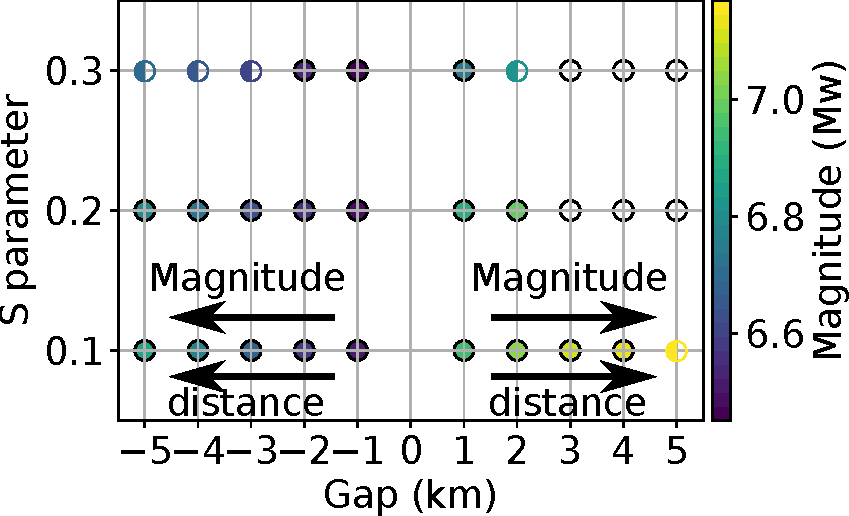
\includegraphics[width=0.9\linewidth]{images/tests_stress} \pause   
  \end{center}
  \vskip -0.4cm
  \begin{itemize}
   \item[\ding{43}] {\scriptsize \textbf{Stress shadow:} \\
                    \vskip 0.1cm
                    The final energy released (M$_w$ proxy) increases/decreases according to the distance between faults.\\
                    \vskip 0.3cm \pause
                    The closer \quad $\longrightarrow$ \quad rupture jump \\ 
                    \pause
                    The closer \quad $\longrightarrow$ \quad less magnitude 
                    }
  \end{itemize}
 \end{minipage}
  
\end{frame}


\begin{frame}
 {Special case: offset $-$2.5 km, gap $\pm$5.0 km}

\begin{center}
    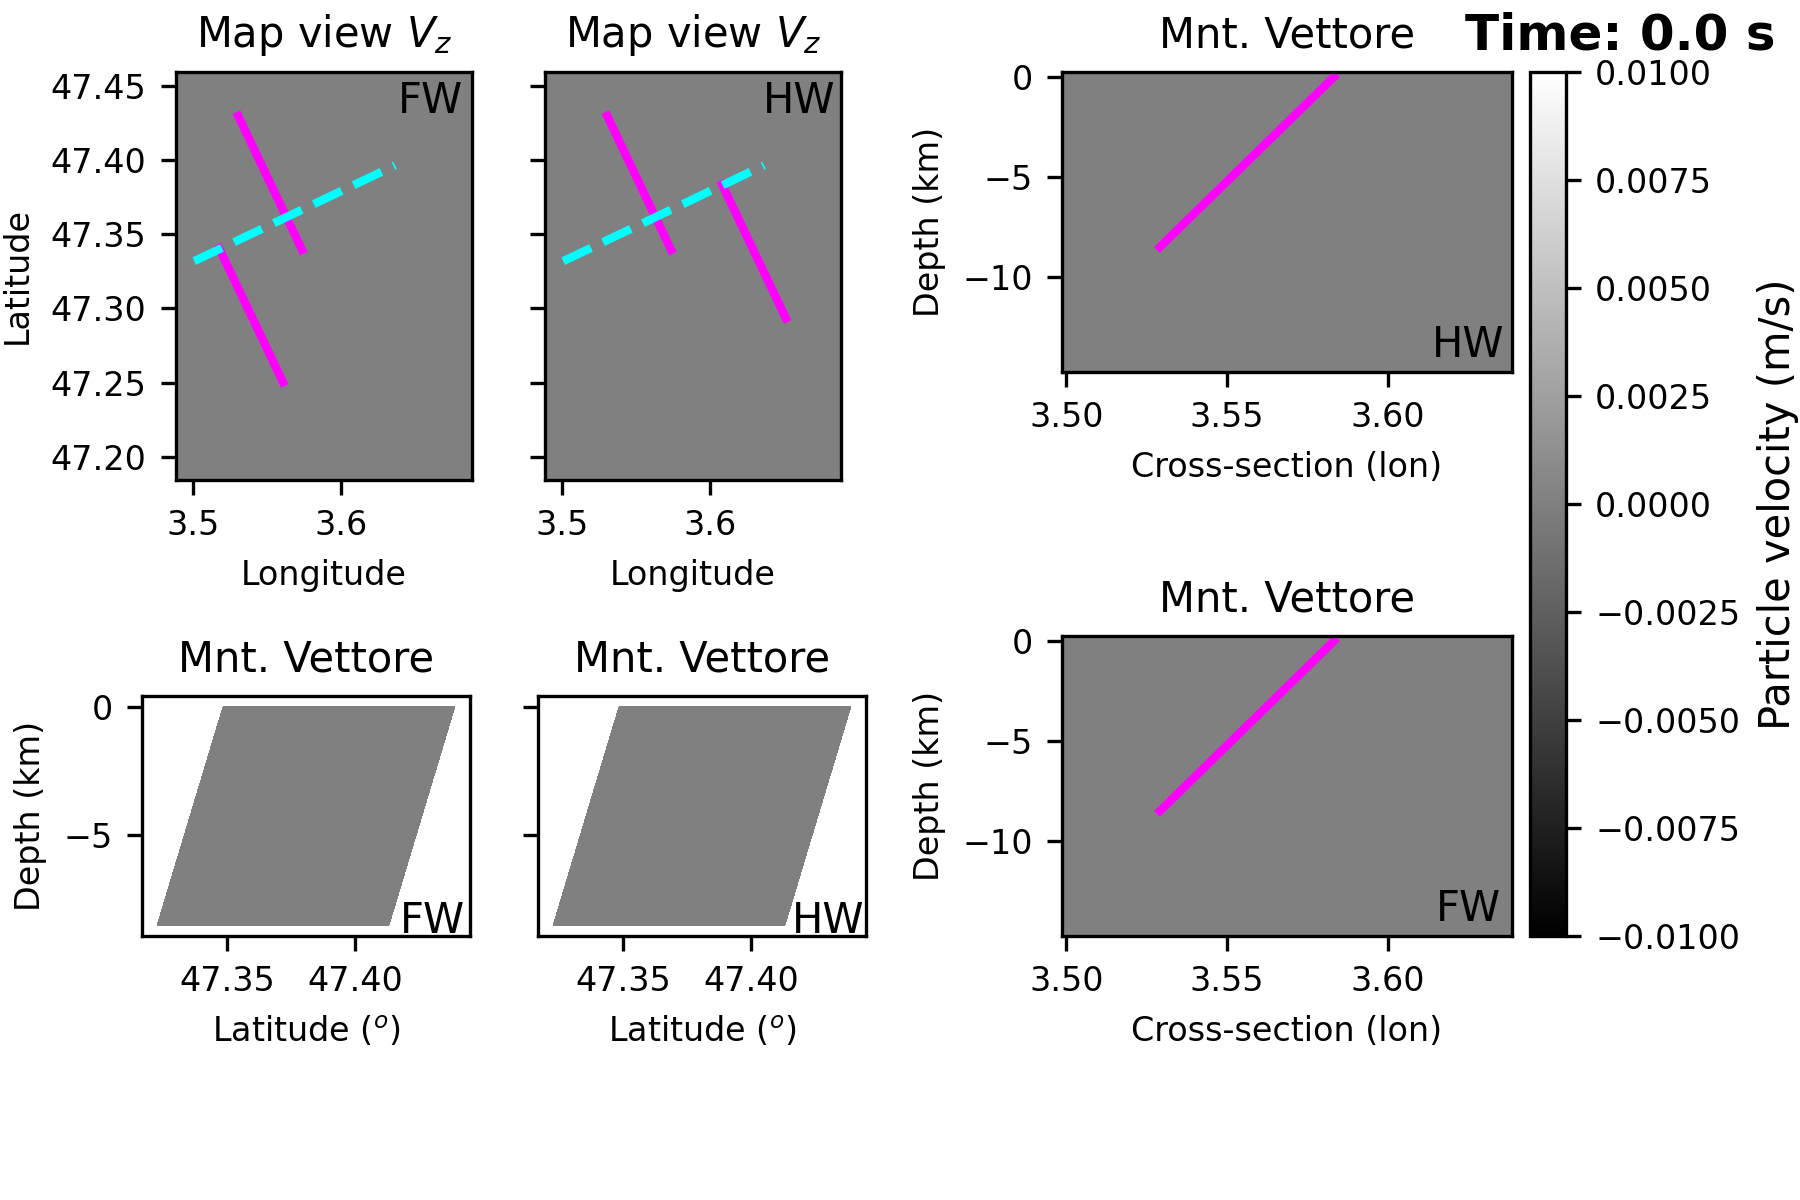
\includegraphics[width=1\linewidth]{images/horizontal_delta_00000}
\end{center}
 
\end{frame}


\begin{frame}
 {Special case: offset $-$2.5 km, gap $\pm$5.0 km}

\begin{center}
    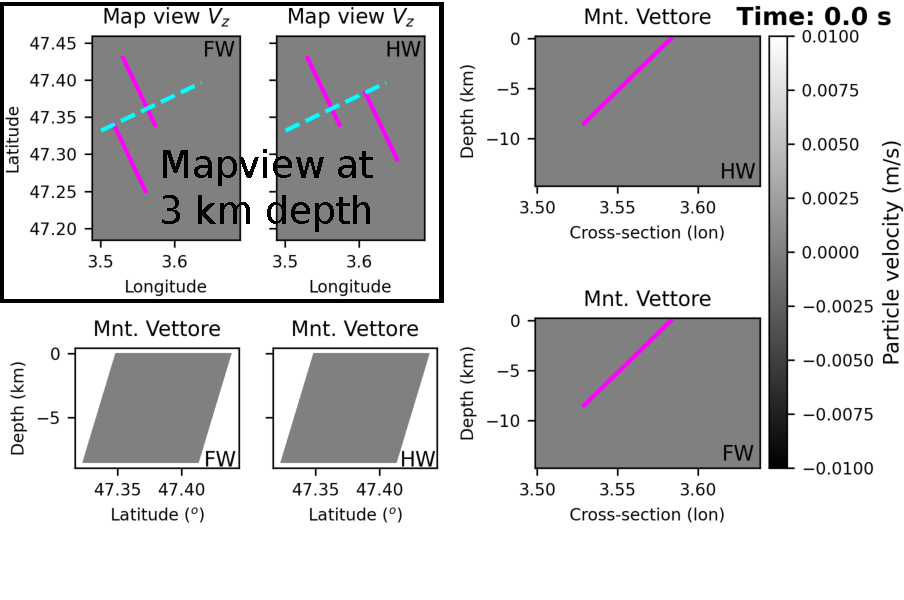
\includegraphics[width=1\linewidth]{images/horizontal_delta_00000a}
\end{center}
\addtocounter{framenumber}{-1}
 
\end{frame}


\begin{frame}
 {Special case: offset $-$2.5 km, gap $\pm$5.0 km}

\begin{center}
    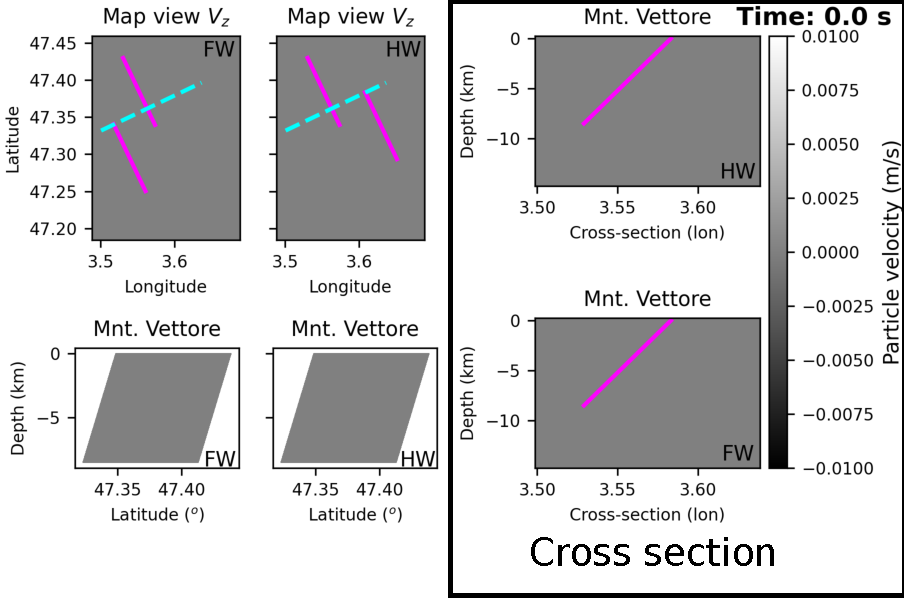
\includegraphics[width=1\linewidth]{images/horizontal_delta_00000b}
\end{center}
\addtocounter{framenumber}{-1}
 
\end{frame}


\begin{frame}
 {Special case: offset $-$2.5 km, gap $\pm$5.0 km}

\begin{center}
    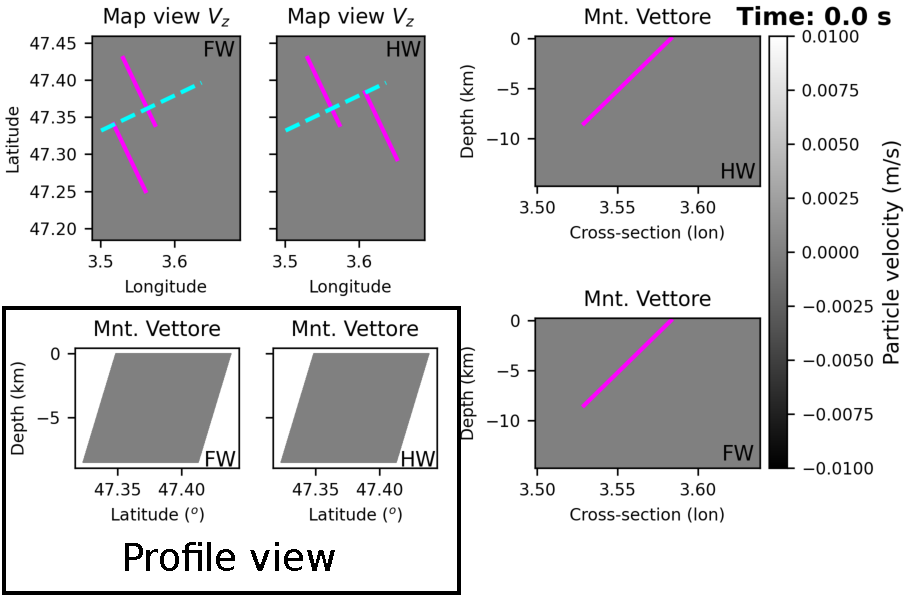
\includegraphics[width=1\linewidth]{images/horizontal_delta_00000c}
\end{center}
\addtocounter{framenumber}{-1}
 
\end{frame}


\begin{frame}
 {Special case: offset $-$2.5 km, gap $\pm$5.0 km}

\begin{center}
%    \animategraphics[
%    label=taylor,
%    loop, autoplay,
%    width=1\linewidth
%    ]{2}{images/video_waves/horizontal_delta_000}{00}{80} 
\end{center}
\addtocounter{framenumber}{-1}
 
\end{frame}


\begin{frame}
 {Special case: offset $-$2.5 km, gap $\pm$5.0 km}

\begin{center}
    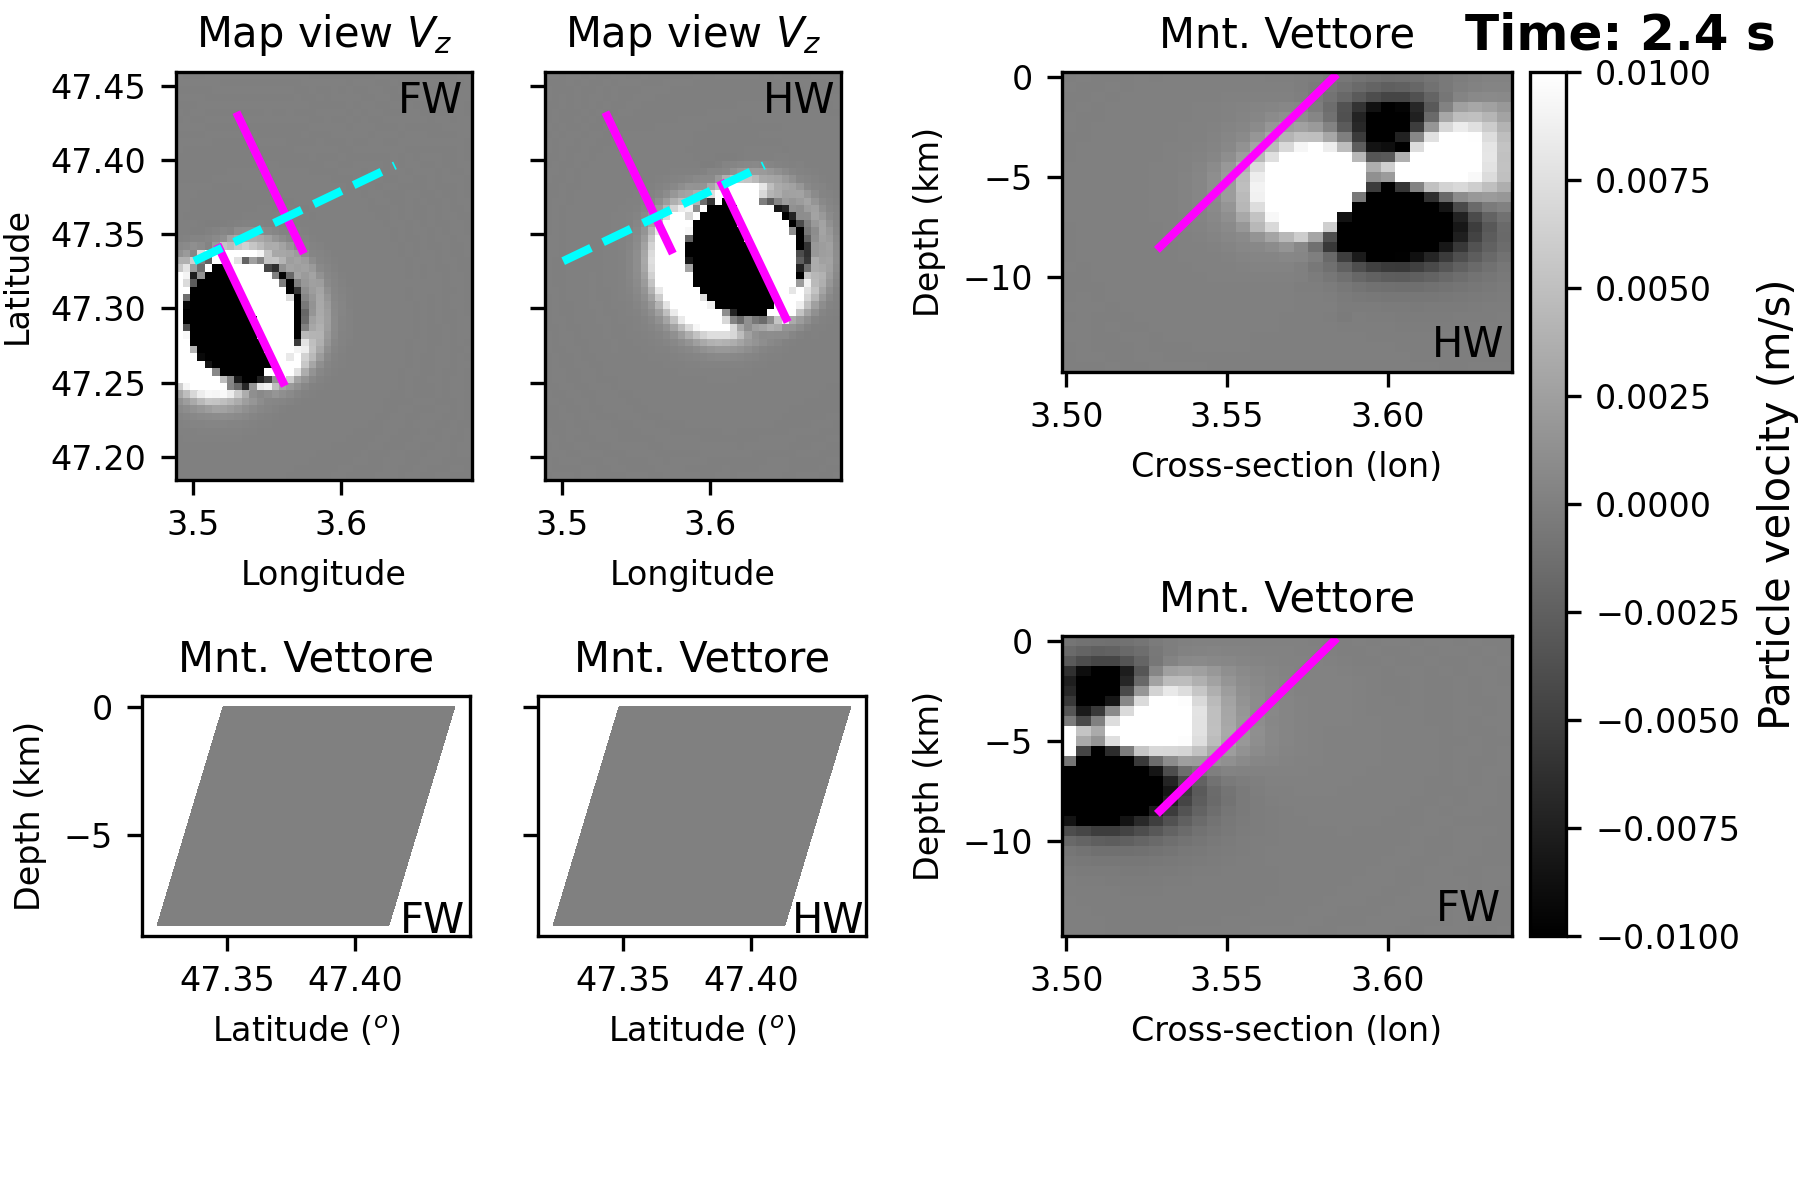
\includegraphics[width=1\linewidth]{images/video_waves/horizontal_delta_00012}
\end{center}
\addtocounter{framenumber}{-1}

\end{frame}


\begin{frame}
 {Special case: offset $-$2.5 km, gap $\pm$5.0 km}

\begin{center}
    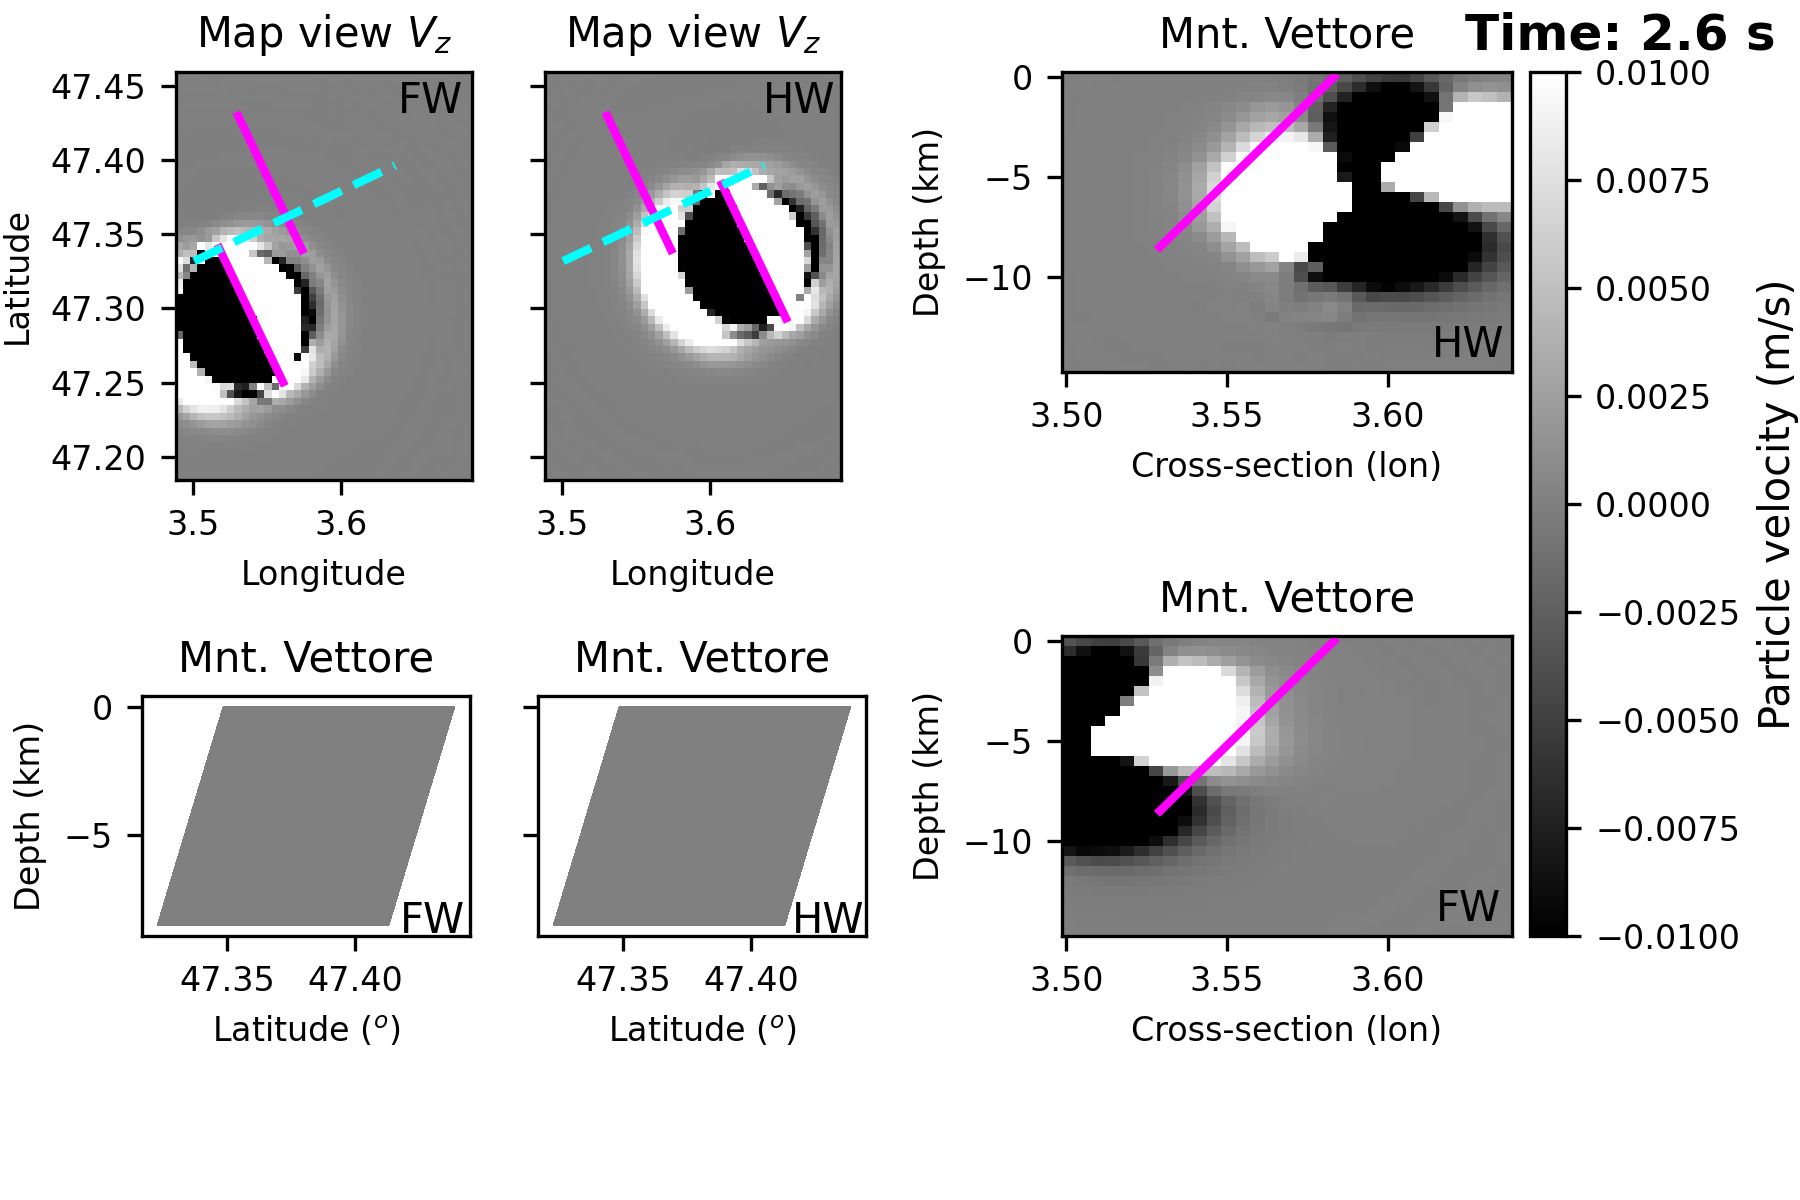
\includegraphics[width=1\linewidth]{images/video_waves/horizontal_delta_00013}
\end{center}
\addtocounter{framenumber}{-1}

\end{frame}


\begin{frame}
 {Special case: offset $-$2.5 km, gap $\pm$5.0 km}

\begin{center}
    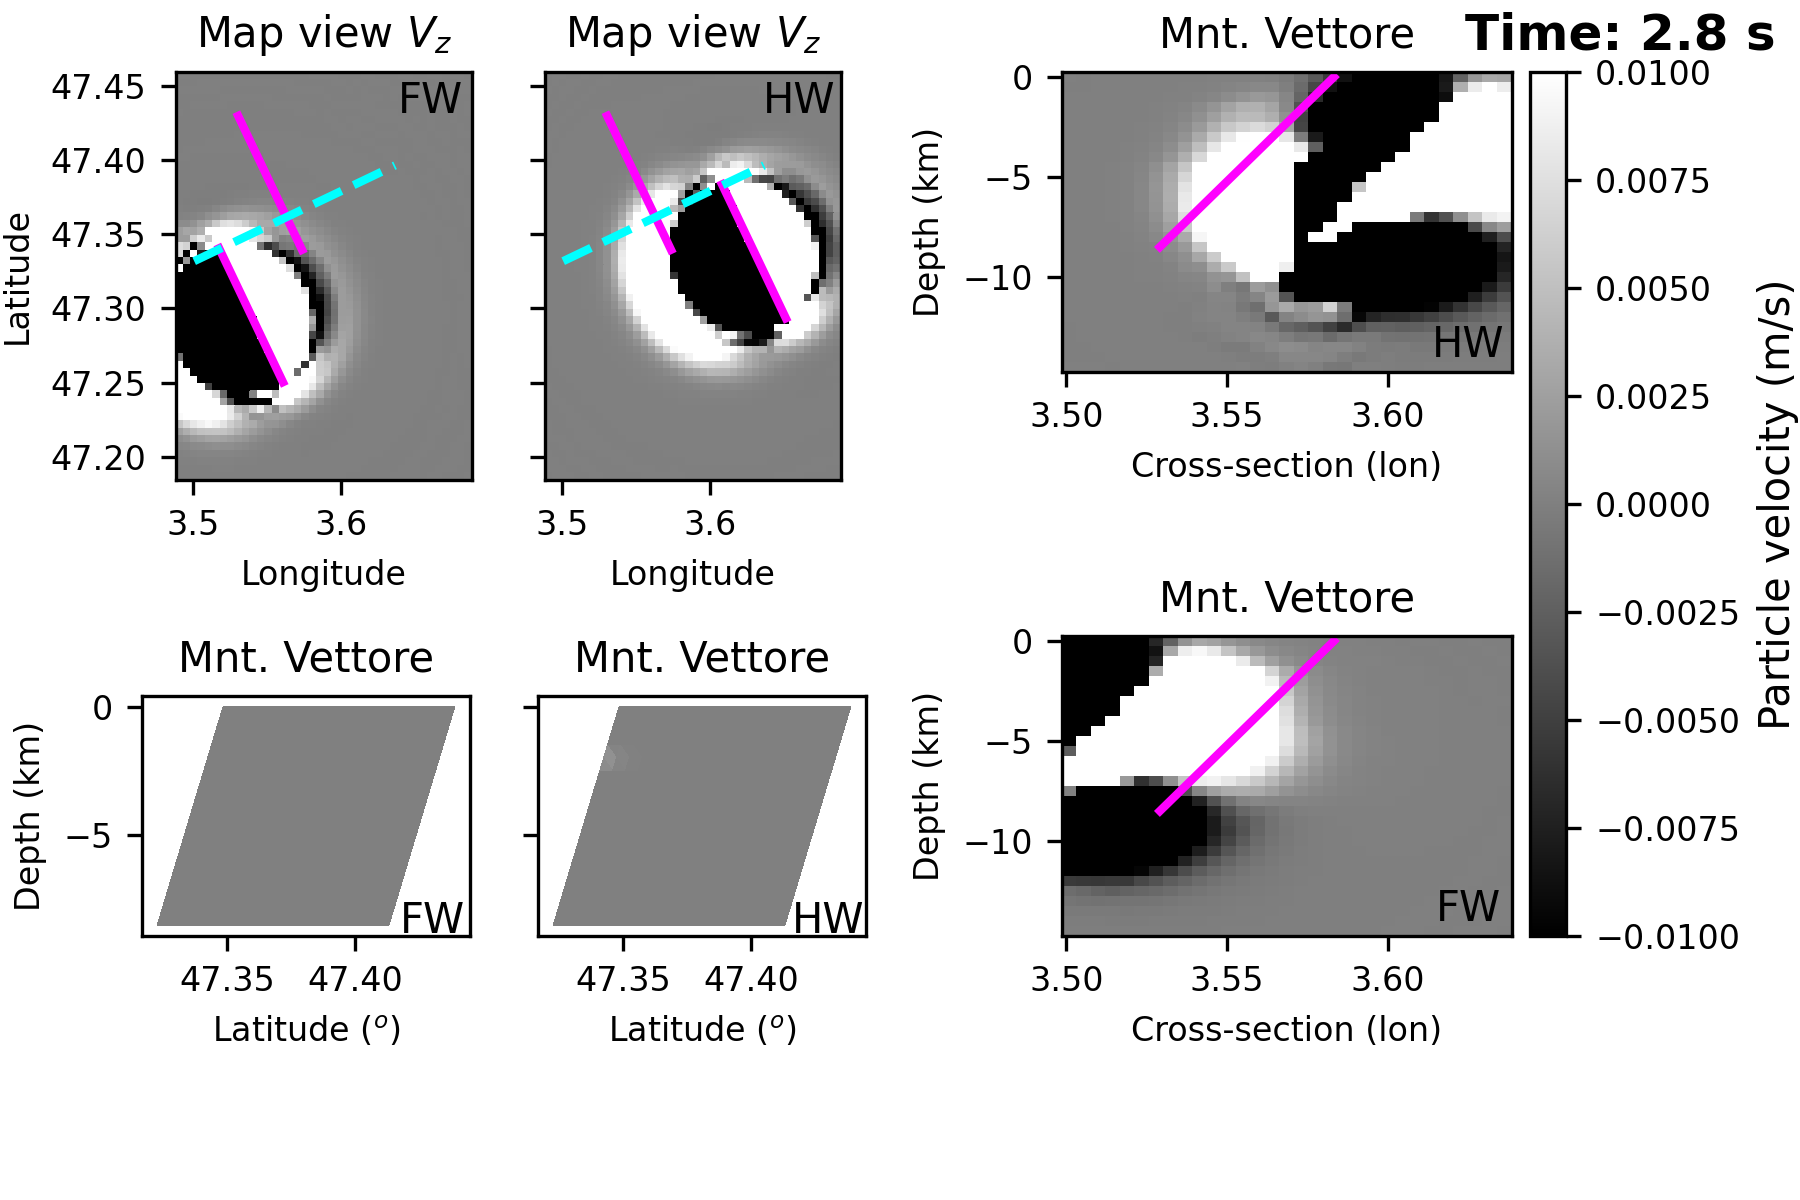
\includegraphics[width=1\linewidth]{images/video_waves/horizontal_delta_00014}
\end{center}
\addtocounter{framenumber}{-1}

\end{frame}


\begin{frame}
 {Special case: offset $-$2.5 km, gap $\pm$5.0 km}

\begin{center}
    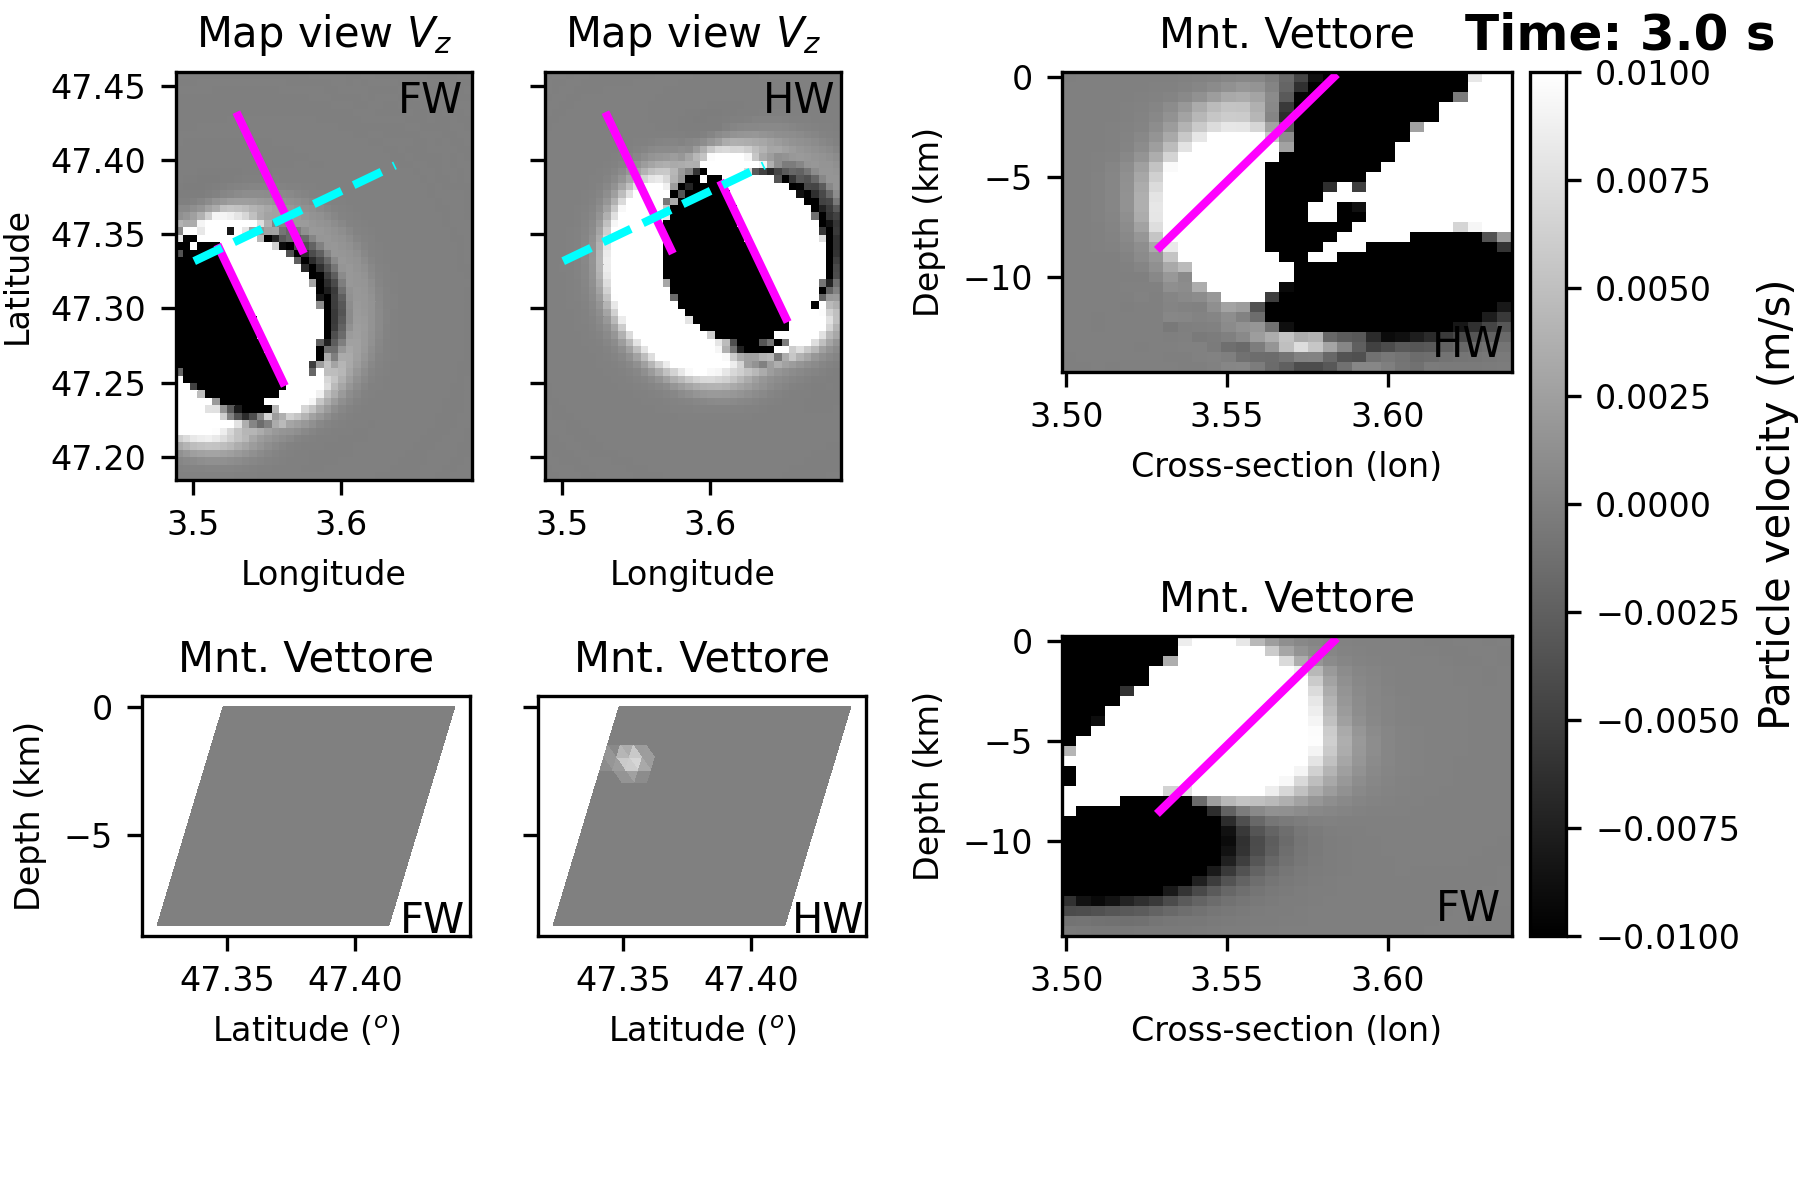
\includegraphics[width=1\linewidth]{images/video_waves/horizontal_delta_00015}
\end{center}
\addtocounter{framenumber}{-1}

\end{frame}

\section{Conclusions}

\begin{frame}
 {Conclusion \& discusion}
 
\textbf{To sum up:} \\ \pause
\vskip 0.3cm
\begin{itemize}
 \item[\ding{43}] \small Static analyses seem to be insufficient to precisely        
                  determine a rupture jump and beak-away behaviors. \pause
                  \vskip 0.1cm
 \item[\ding{43}] \small It is necessary to have an enough large area where
                  $\Delta$CFF$>$0 to ensure a sustained rupture after it jumped across the step-over. \pause
                  \vskip 0.1cm
 \item[\ding{43}] \small Behaviors such as ``stress shadow" and ''asymmetric            
                  response" were observed as for strike-slip faults. \pause
                  \vskip 0.1cm
  \item[\ding{43}] \small The 2nd fault rupture seems to be dynamically 
                   triggered by the strong stopping phase arriving from behind. \pause
                  \vskip 0.1cm
  \item[\ding{43}] \small 5 km seems to be the largest distance that the
                   rupture can jump (considering very high stress levels).
\end{itemize}

\centering \LARGE Thank you for listening! \\ Questions?
 
\end{frame}



\section*{References}
\begin{frame}

    {\tiny \bibliography{\dirbiblio/bibliography} }							\bibliographystyle{apalike}    

\end{frame}


\end{document}

